%\begin{savequote}[8cm]
%\textlatin{Neque porro quisquam est qui dolorem ipsum quia dolor sit amet, consectetur, adipisci velit...}
%
%There is no one who loves pain itself, who seeks after it and wants to have it, simply because it is pain...
%  \qauthor{--- Cicero's \textit{de Finibus Bonorum et Malorum}}
%\end{savequote}

\chapter{\label{ch:3-detector}The LHCb detector} 

%\minitoc

The Large Hadron Collider (LHC) is the world's largest and most powerful particle accelerator, located near Geneva, Switzerland. The LHC ring is 27~km in circumference, located 100~m underground and consists of a series of superconducting magnets and accelerating modules to boost the particle energy. Two high energy proton or heavy ion beams travel in opposite directions at energies up to $\sqrt{s}=13~\tev$. The protons are obtained by ionising hydrogen atoms, these protons are accelerated in stages through various parts of the LHC accelerator complex, as shown in \fig\ref{lhcdiagram}. Firstly, the protons are accelerated in Linac 2 to energies of 50\mev, followed by the Proton Synchrotron Booster (PSB), the Proton Synchrotron (PS) and the Super Proton Synchrotron (SPS), accelerating the protons to 1.4~\gev, 25~\gev and 450~\gev respectively. Finally, the protons are injected into the LHC. Two proton beams are injected in opposite directions, reaching energies of up to $\sqrt{s}=13~\tev$, and focused to collide at four locations around the LHC ring. These locations are where the four main particle physics detectors are located: the Large Hadron Collider beauty (\lhcb) experiment as well as \atlas, \cms and \alice.

\begin{figure}
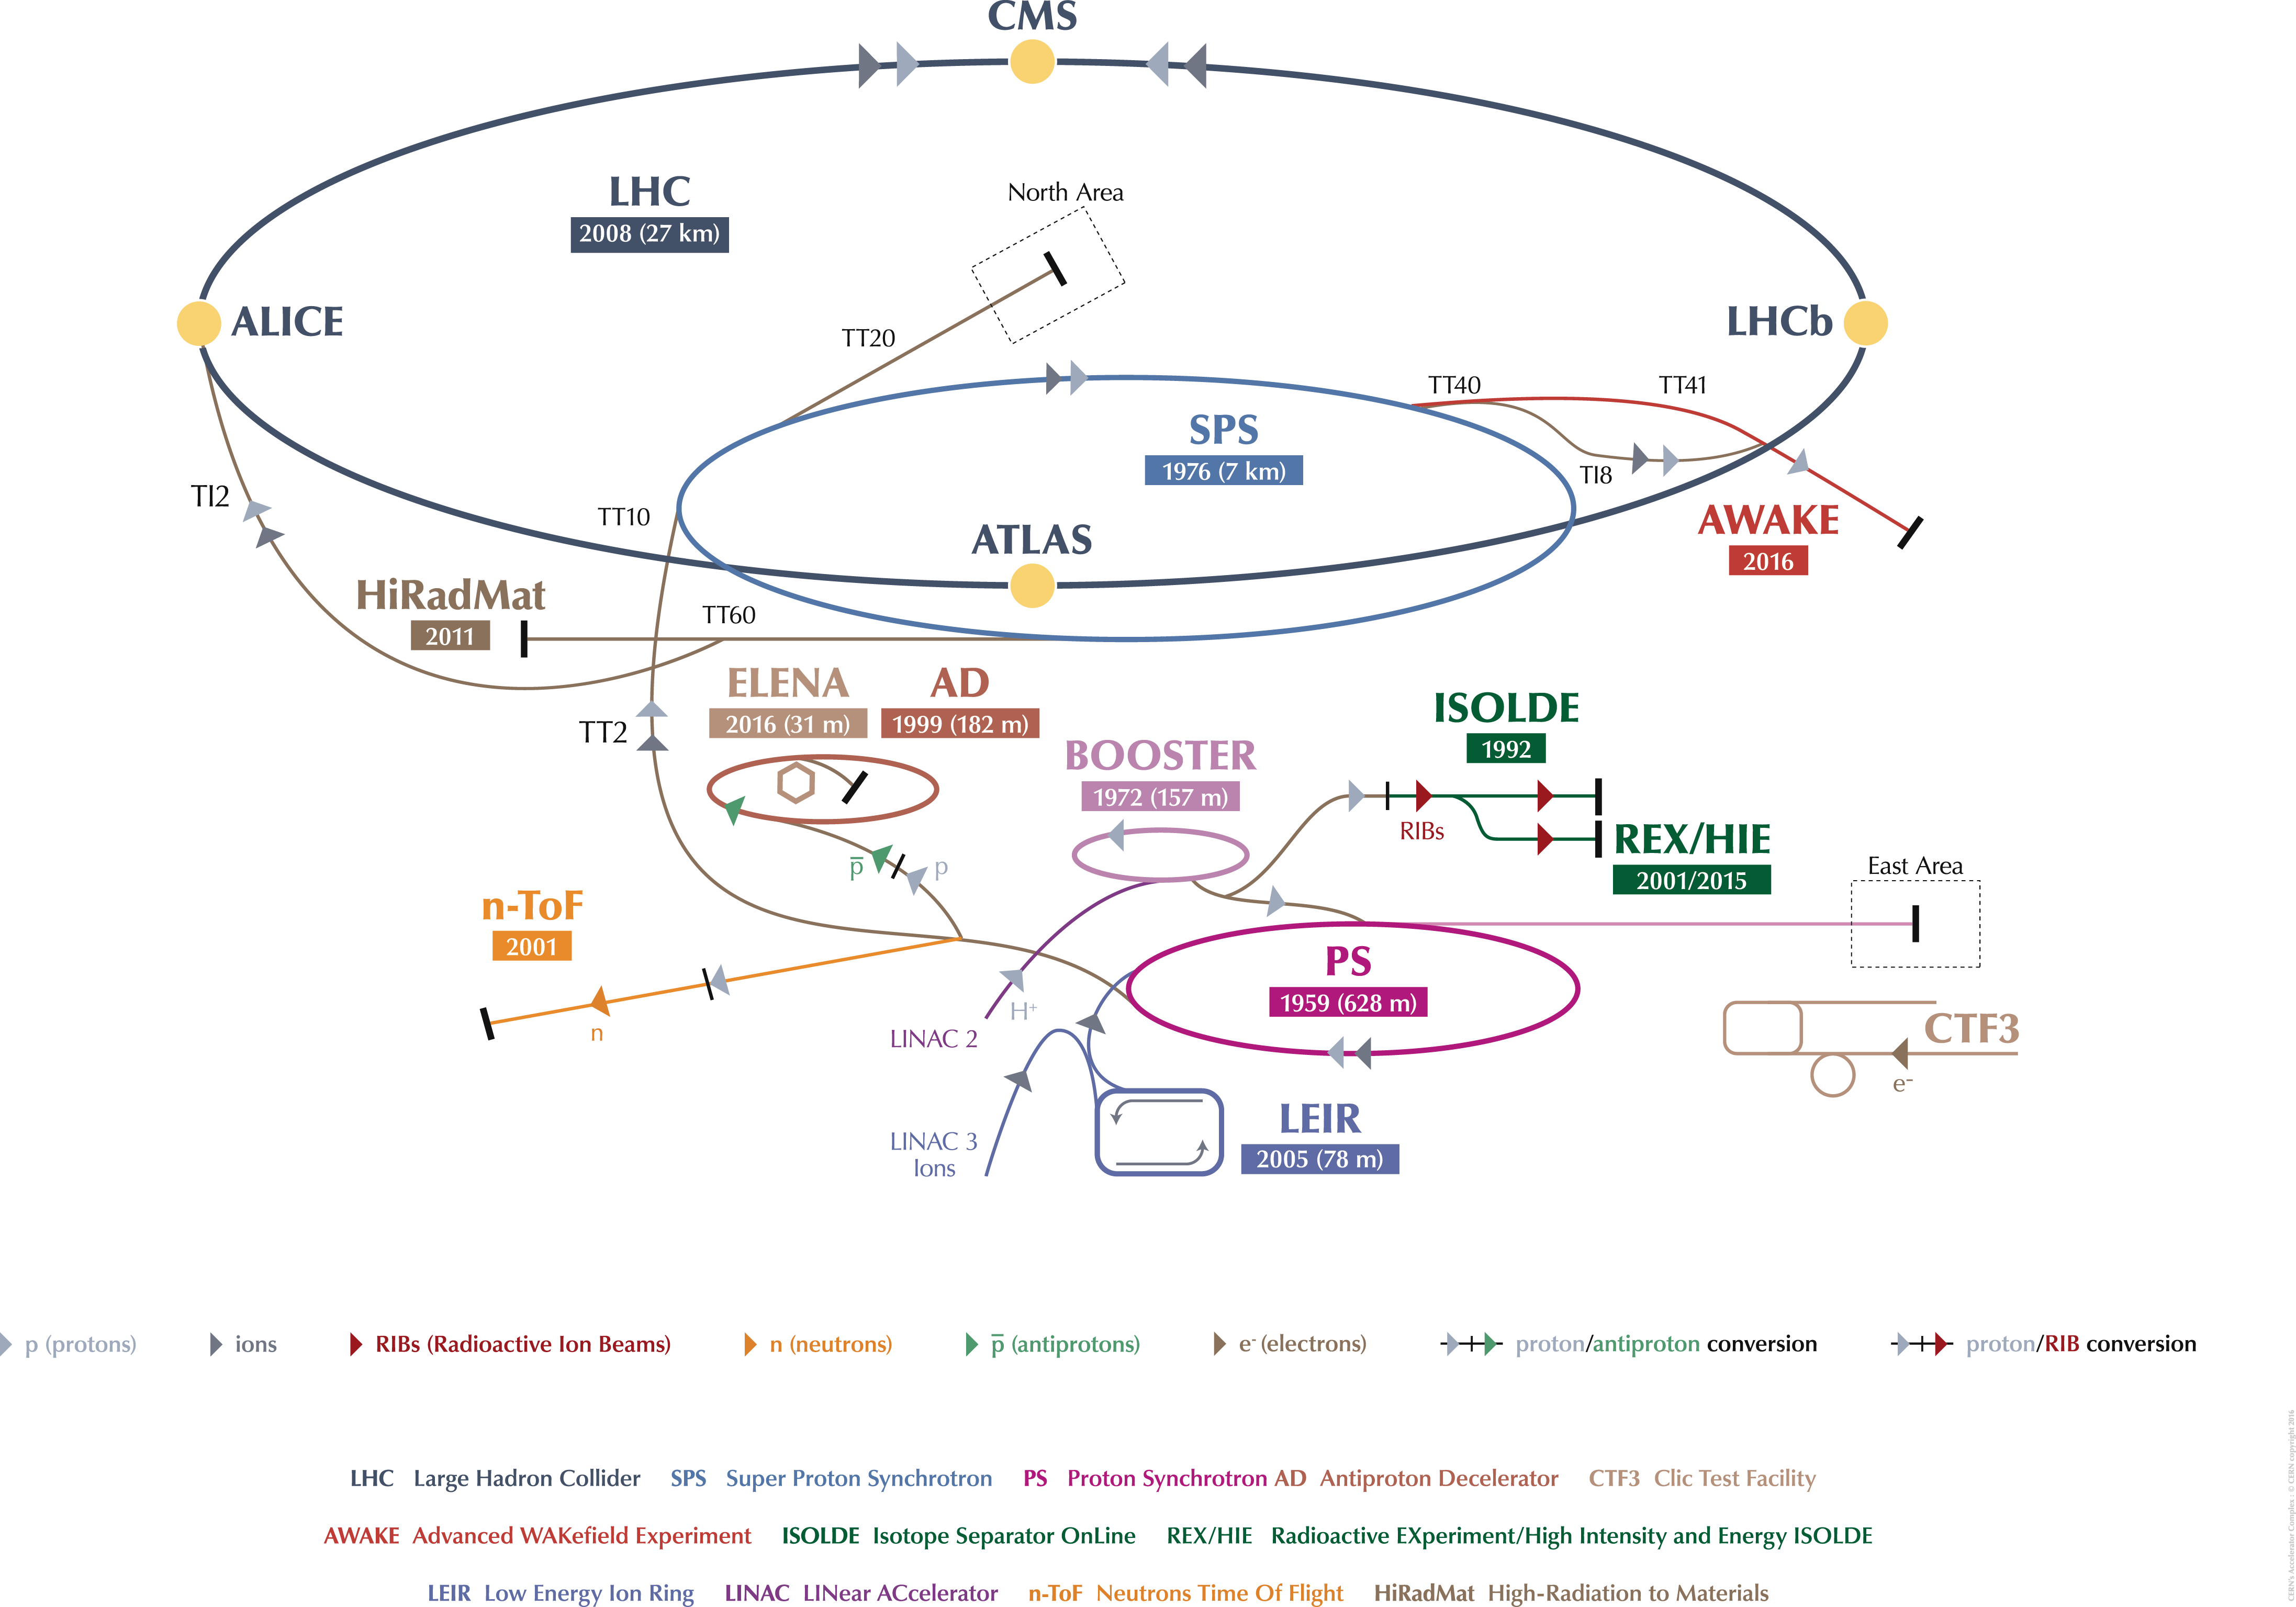
\includegraphics[trim = 0mm 70mm 0mm 0mm,clip,width=\linewidth]{figures/detector/CCC-v2016.png}
\caption{Diagram of the LHC accelerator complex.}
\label{lhcdiagram}
\end{figure}

There have been two major data taking periods of the \lhc, named \runone and \runtwo. \runone occurred between 2010 and 2012, where the centre of mass energy was $\sqrt{s}=$7~\tev (2010 and 2011) and 8~\tev (2012). Data collection for \runtwo began in 2015 and is due to end in 2018, with $\sqrt{s}=$13~\tev. At LHCb the collision conditions are designed to have roughly one proton-proton ($pp$) interaction per bunch crossing in order to allow effective primary vertex selection, necessary for the study of \B and \D meson decays, efficient track finding, and reduced radiation damage and detector occupancy. The low luminosity running is achieved by a process called {\textit{luminosity levelling}}, which involves reducing the transverse overlap of the two beams in order to reduce the area available for interactions. This allows the peak luminosity and number of $pp$ interactions per bunch crossing to be optimal, while maximising the integrated luminosity. Most of the LHCb data were recorded at an instantaneous luminosity of $4 \times 10^{32}\text{cm}^{-2}\text{s}^{-1}$, with an average of 1.7 $pp$ collisions per bunch crossing for \runone and 1.1 for \runtwo. In \runone collisions occurred at a frequency of 20 MHz, corresponding to collisions every 50~\ns, which increased to a bunch crossing rate of 40 MHz in \runtwo.

This thesis uses the complete 3~\invfb \runone dataset corresponding to 1~\invfb of $\sqrt{s} = $7~\tev data recorded in 2011 and 2~\invfb of $\sqrt{s} = $8~\tev data recorded in 2012, as well as 1.8~\invfb of the \runtwo dataset, corresponding to all of the data recorded in 2015 and 2016 at $\sqrt{s}=$13~\tev.

The \lhcb detector is designed to study particles containing \bquark and \cquark quarks. These quarks are produced dominantly via gluon interactions. The gluons typically have highly asymmetric momenta, therefore the \bquark\bquarkbar quark pair is produced predominantly in the forward (or backward) direction, illustrated in \fig\ref{bbar}. For this reason, the \lhcb detector~\cite{Alves:2008zz,LHCb-DP-2014-002} was designed as a single-arm forward spectrometer, as shown in \fig\ref{lhcbdetector}. It covers the \mbox{pseudorapidity} range $2<\eta <5$, where the pseudorapidity, $\eta$, is defined as
\begin{equation}
\eta \equiv -\ln \left[ \tan \left( \frac{\theta}{2} \right) \right] \text{ ,}
\end{equation}
where $\theta$ is the angle between the particle's momentum vector and the beam axis. This angular region captures 25\% of all \bquark\bquarkbar pairs produced. The detector is described using a right-handed coordinate system, where $z$ represents the direction of the beam into the spectrometer, $x$ points outwards from the centre of the ring and $y$ points upwards. The \lhcb spectrometer has an angular acceptance up to 300~mrad in the horizontal plane, and 250~mrad in the vertical plane. It is composed of many sub-detectors that are each specialised for a specific role. These are the Vertex Locator (\velo), the Ring Imaging Cherenkov detectors (RICH1 and RICH2), the Tracker Turicensis (TT), the dipole magnet, the tracking stations T1-T3, the calorimeter system (SPD/PS, ECAL, HCAL) and the muon stations M1-M5. In Secs.~\ref{sec:detector:velo} to \ref{sec:detector:muon}, individual descriptions of these sub-detectors are presented.

\begin{figure}
\centering
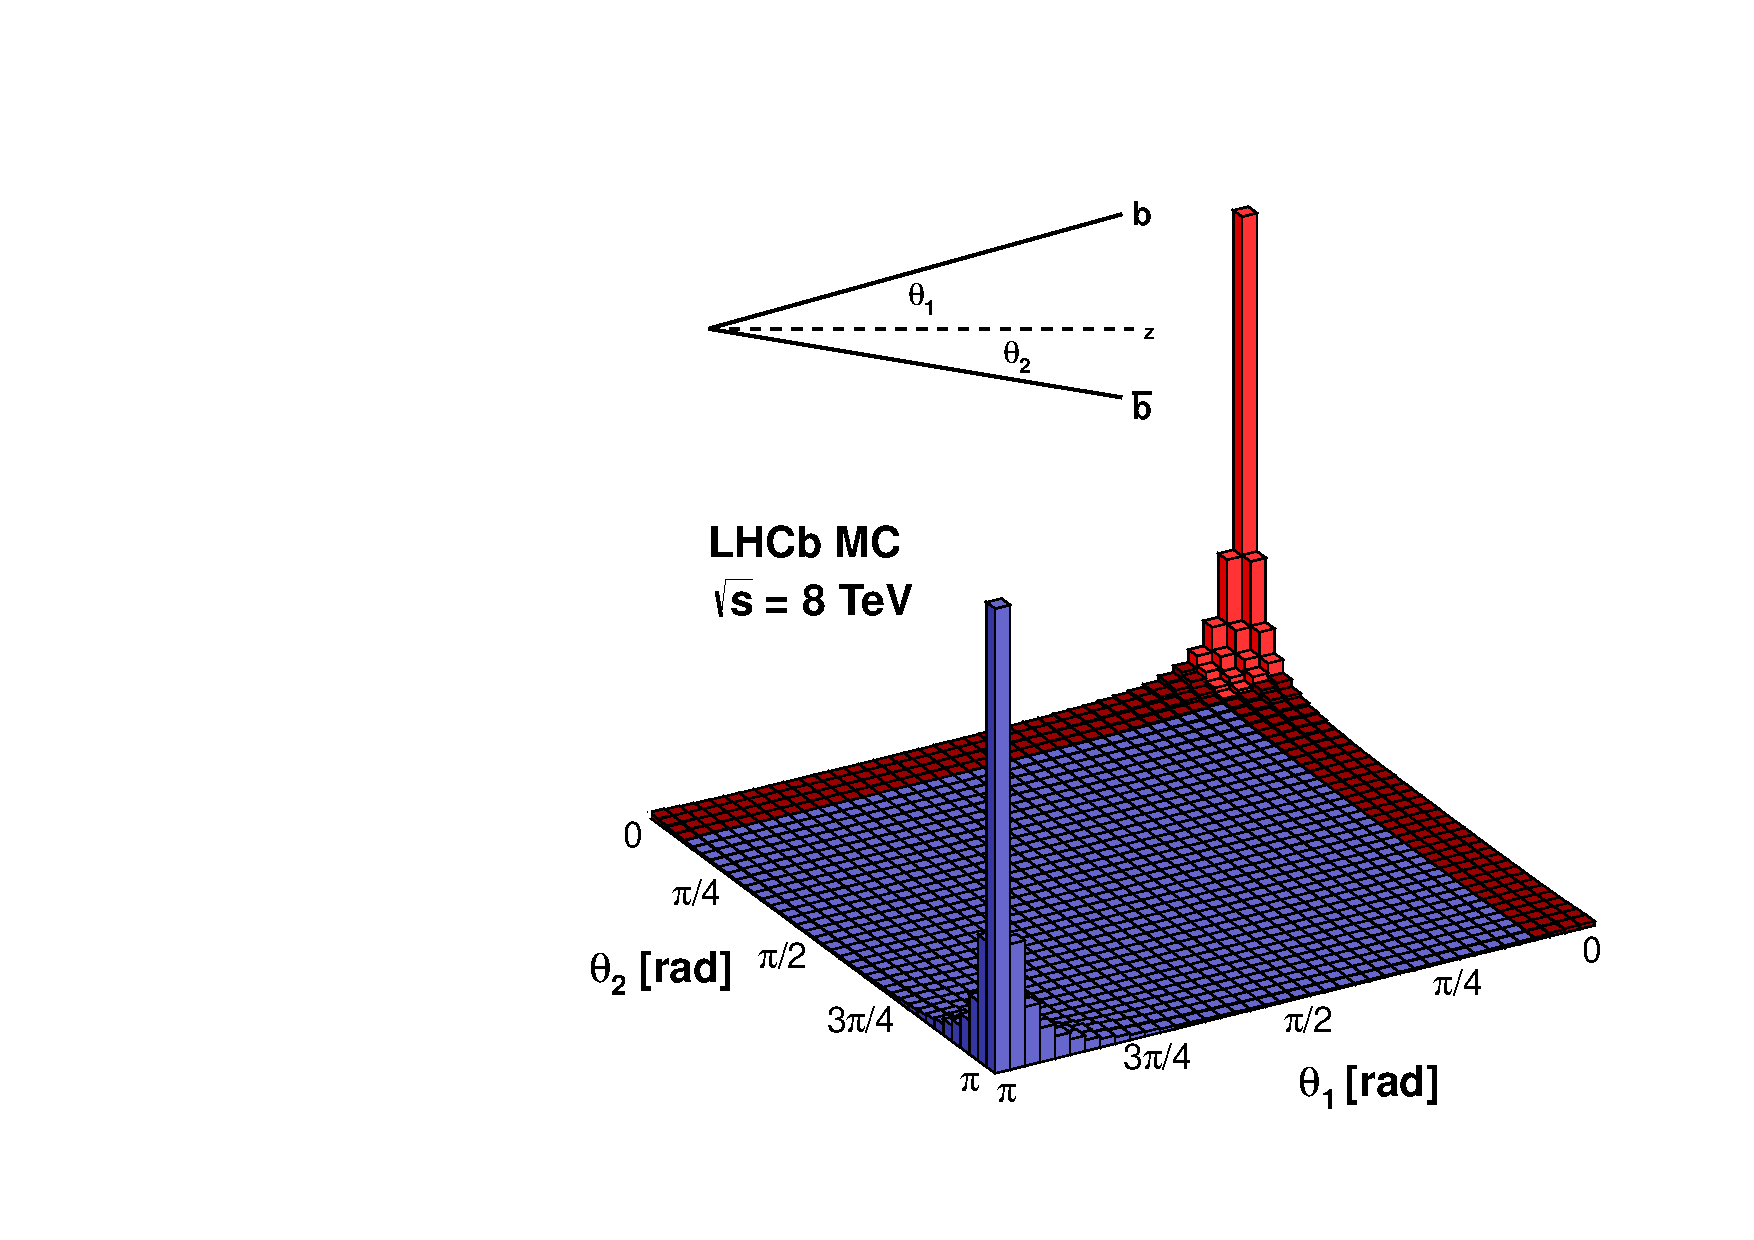
\includegraphics[width=0.5\linewidth]{figures/detector/08_rad_acc_scheme_right.pdf}
\caption{The distribution of \bquark\bquarkbar quark pair productions in simulated $pp$ collisions at 8~TeV as a function of the polar angles $\theta_1$ and $\theta_2$ with respect to the beam axis, $z$. The red shading indicates the region covered by the \lhcb detector.}
\label{bbar}
\end{figure}

\begin{figure}
\includegraphics[width=\linewidth]{figures/detector/lhcb.pdf}
\caption{Diagram of the \lhcb detector. The various sub-detectors are the Vertex Locator (\velo), the Ring Imaging Cherenkov detectors (RICH1 and RICH2), the Tracker Turicensis (TT), the dipole magnet, the tracking stations T1-T3, the calorimeter system (SPD/PS, ECAL, HCAL) and the muon stations M1-M5.}
\label{lhcbdetector}
\end{figure}

\section{The Vertex Locator}
\label{sec:detector:velo}

The Vertex Locator (\velo)~\cite{LHCb-DP-2014-001} provides precise tracking close to the \lhcb interaction region to identify primary and secondary vertices from heavy-flavour decays, which is essential for studies of long-lived particles such as \B and \D mesons. The \velo is a silicon microstrip detector situated around the $pp$ interaction point, referred to as the primary vertex (PV). It consists of 42 silicon modules arranged along the beam, each providing a measurement of the radial coordinate, $r$, and azimuthal coordinate, $\phi$, using so-called $R$ sensors and $\Phi$ sensors respectively, shown in \fig\ref{velolayout}. The sensors are located 7~\mm from the LHC beams at their closest points. The \velo modules are retracted 29~\mm in the horizontal direction during injection of the LHC beams in order to reduce radiation damage and returned to their nominal position during stable beams. The sensors are enclosed in a secondary vacuum envelope which is separated from the LHC vacuum by corrugated foil sheets designed to protect the \velo modules against electromagnetic interference from the LHC beams.

\begin{figure}
\centering
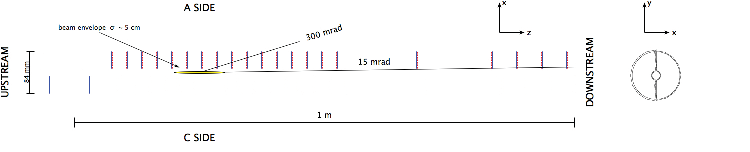
\includegraphics[width=\linewidth]{figures/detector/VELO_detector_layout_crop.pdf}
\hfill
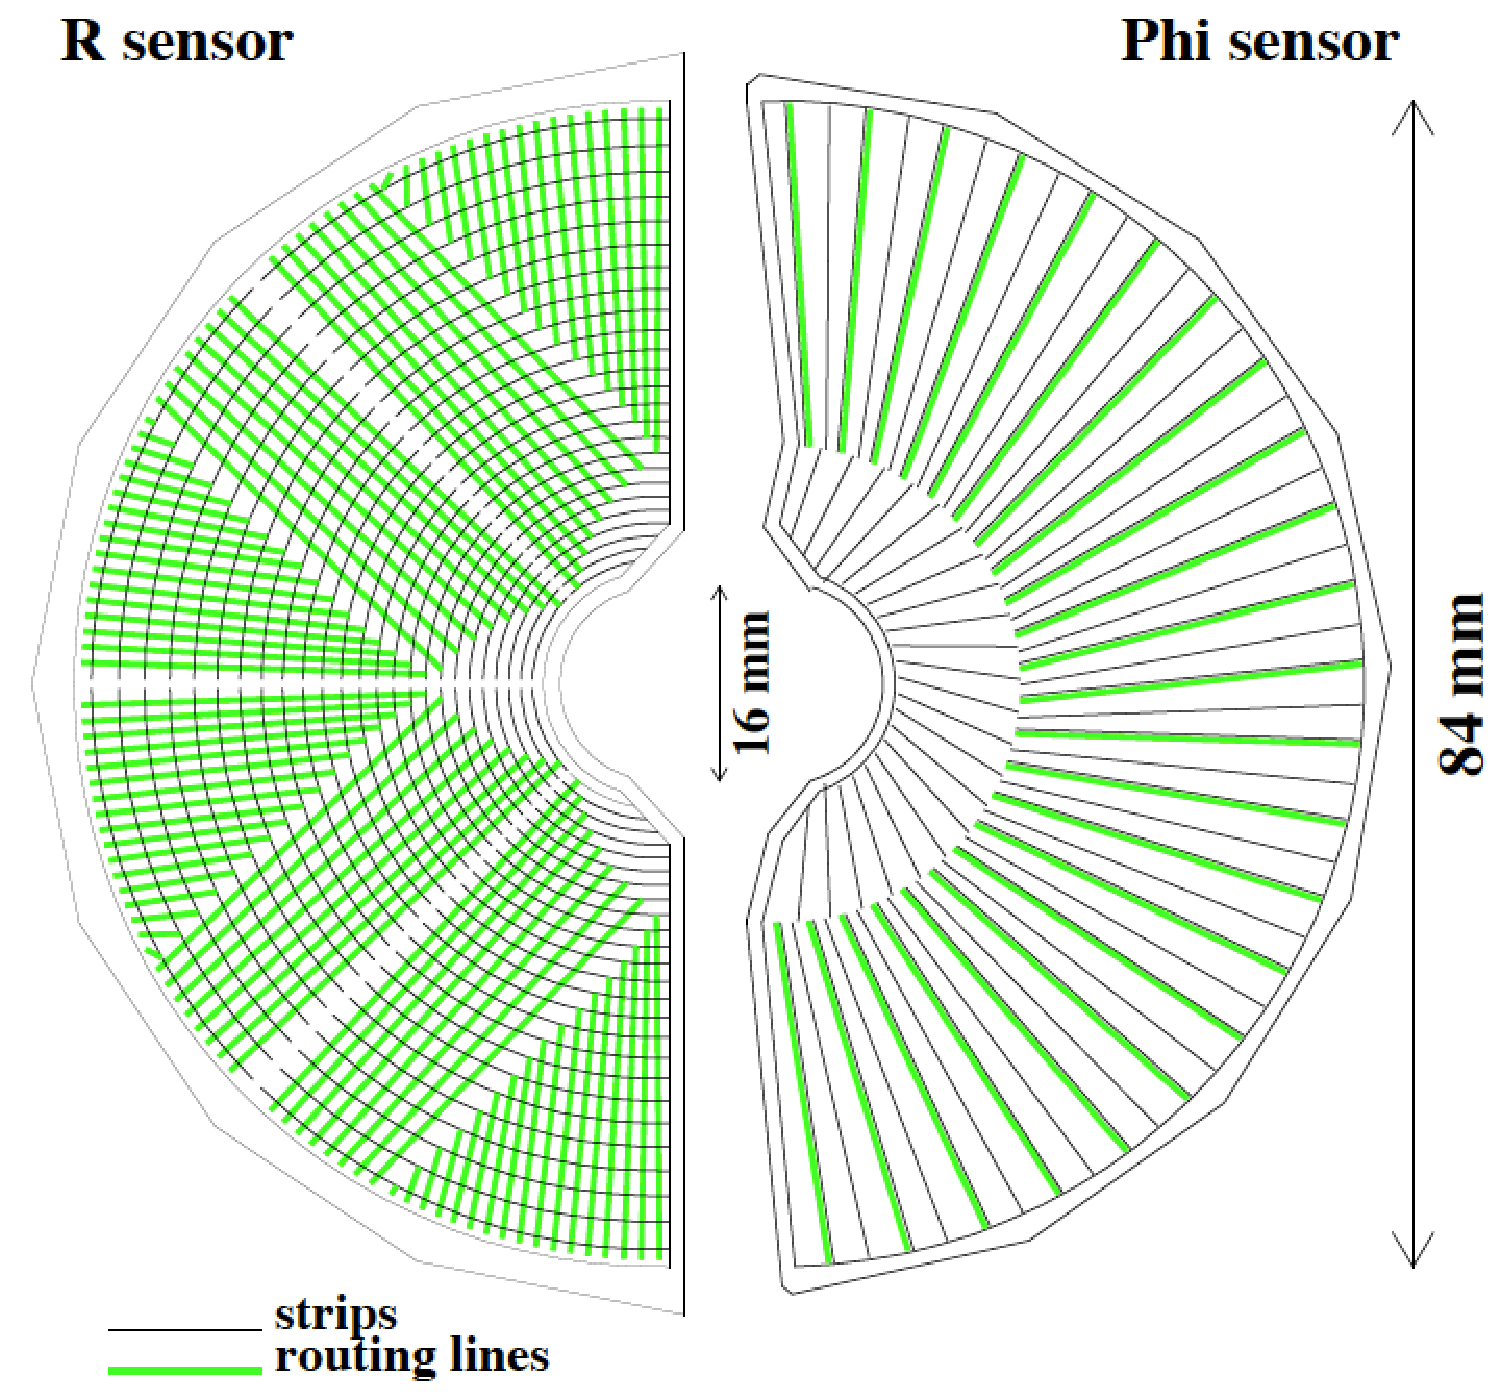
\includegraphics[width=0.3\linewidth]{figures/detector/randphisensors.pdf}
\caption{Layout of the \velo detector (top). Schematic diagram showing the $R$ and $\Phi$ sensors (bottom). Reproduced from Ref.~\cite{LHCb-DP-2014-002}.}
\label{velolayout}
\end{figure}

The \velo has a high spatial resolution, enabling precise determination of a particle's flight direction close to the primary interaction point. The impact parameter (IP) of a track is defined as the distance between the track and the PV at the track's point of closest approach to the PV. Long-lived \B and \D mesons studied in this thesis have their decay vertices displaced from the PV and as such tend to have a large IP. Therefore, the performance of the \velo can be quantified by the IP resolution, which, determined from 2012 data, is less than 35\mum for particles with transverse momentum greater than 1~\gevc~\cite{LHCb-DP-2014-001}. The IP resolution in the $x$ and $y$ directions as a function of track momentum is shown in \fig\ref{veloperformance}. The vertex resolution of the \velo is 13~\mum in the transverse plane and 71~\mum along the beam axis for vertices with 25 tracks~\cite{LHCb-DP-2014-001}.

\begin{figure}
\centering
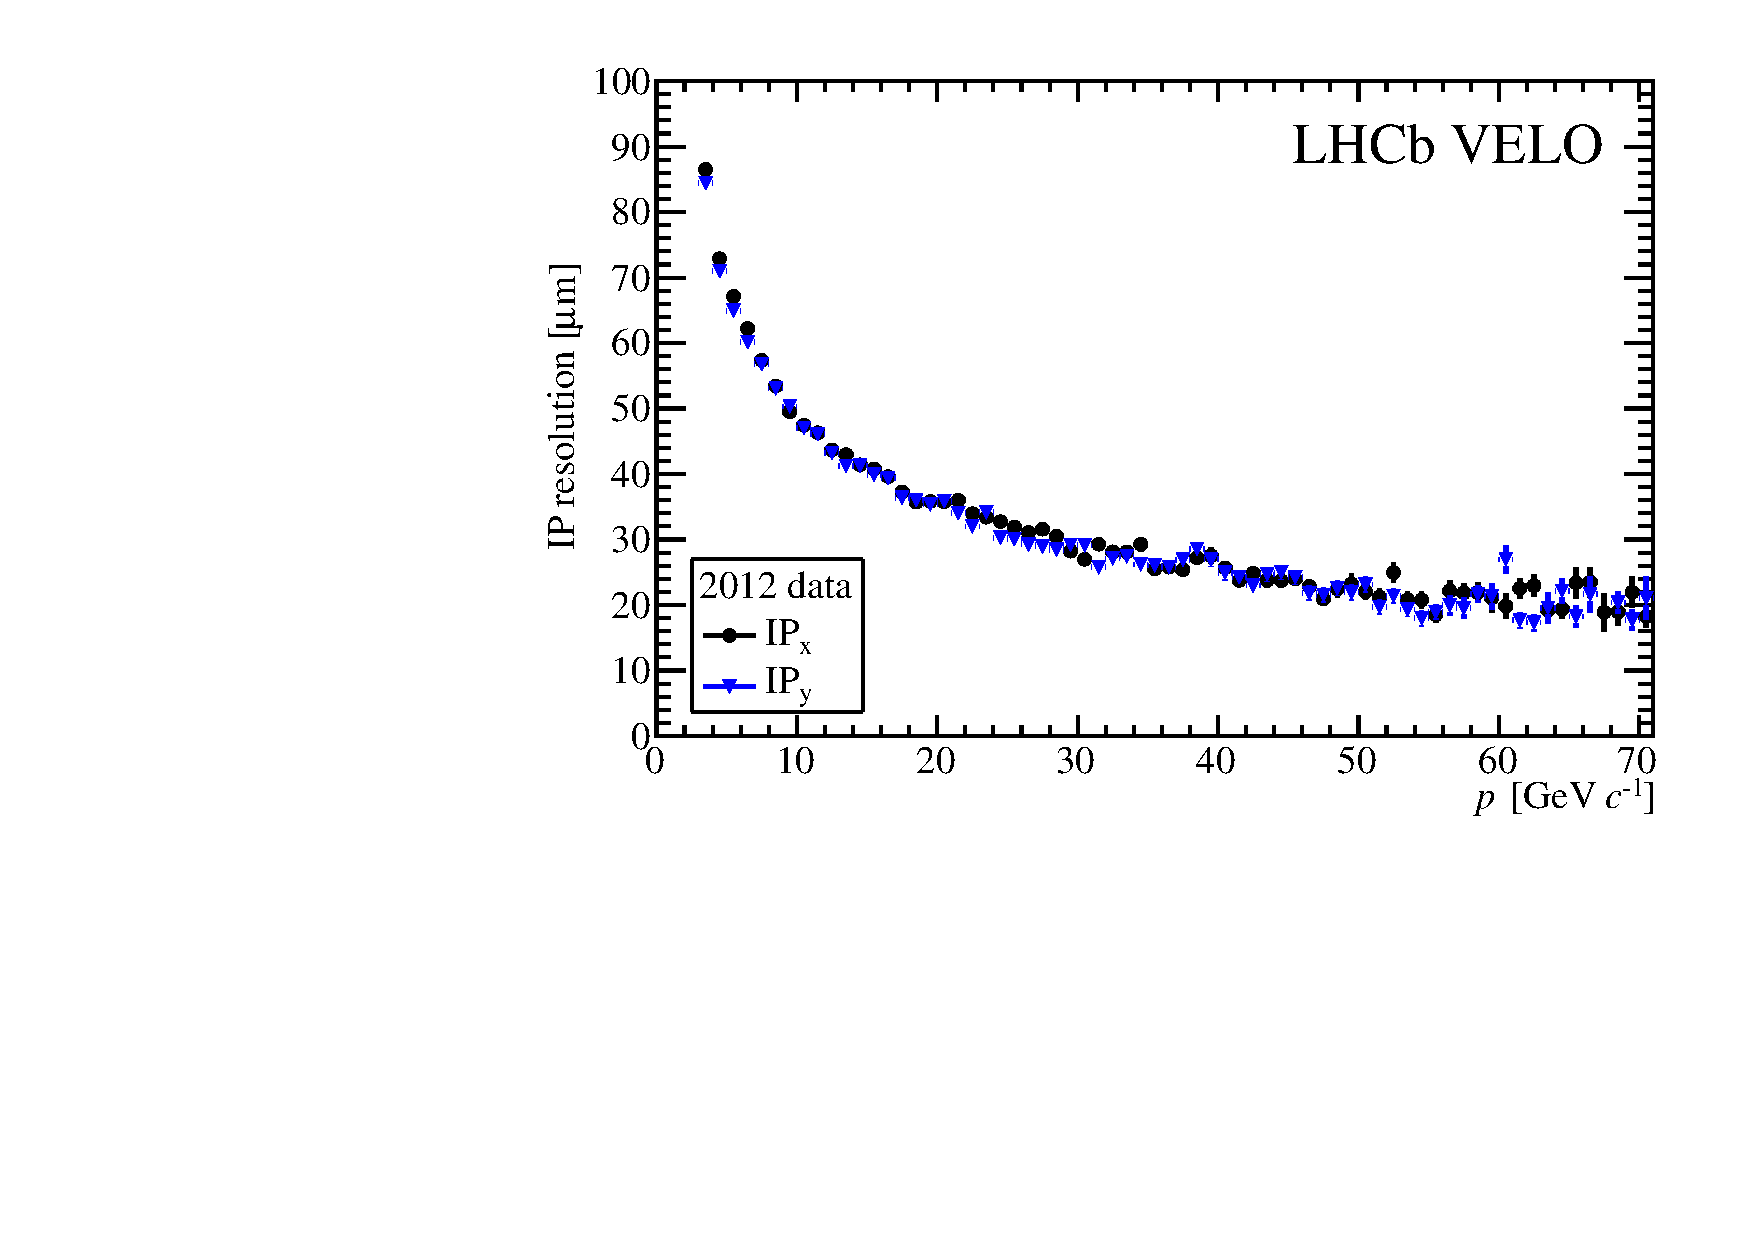
\includegraphics[width=0.5\linewidth]{figures/detector/IPRes-Vs-P-CompareIPxIPy-2012.pdf}
\caption{IP resolution as a function of momentum in both the $x$ and $y$ directions. Reproduced from Ref.~\cite{LHCb-DP-2014-001}.}
\label{veloperformance}
\end{figure}

\section{Tracking and magnet}
\label{sec:detector:tracking}

The \lhcb tracking system consists of the \velo and four planar tracking stations further downstream: the Tracker Turicensis (TT), made of silicon microstrips, upstream of the dipole magnet and tracking stations T1-T3 downstream of the magnet, as shown in \fig\ref{tracking}. The tracking stations T1-T3 have an inner region (Inner Tracker, IT) consisting of the same silicon microstrips as the TT and an outer region (Outer Tracker, OT) consisting of straw tubes. Charged particles require a minimum momentum of 1.5~\gevc to reach the tracking stations T1-T3.

\begin{figure}
\centering
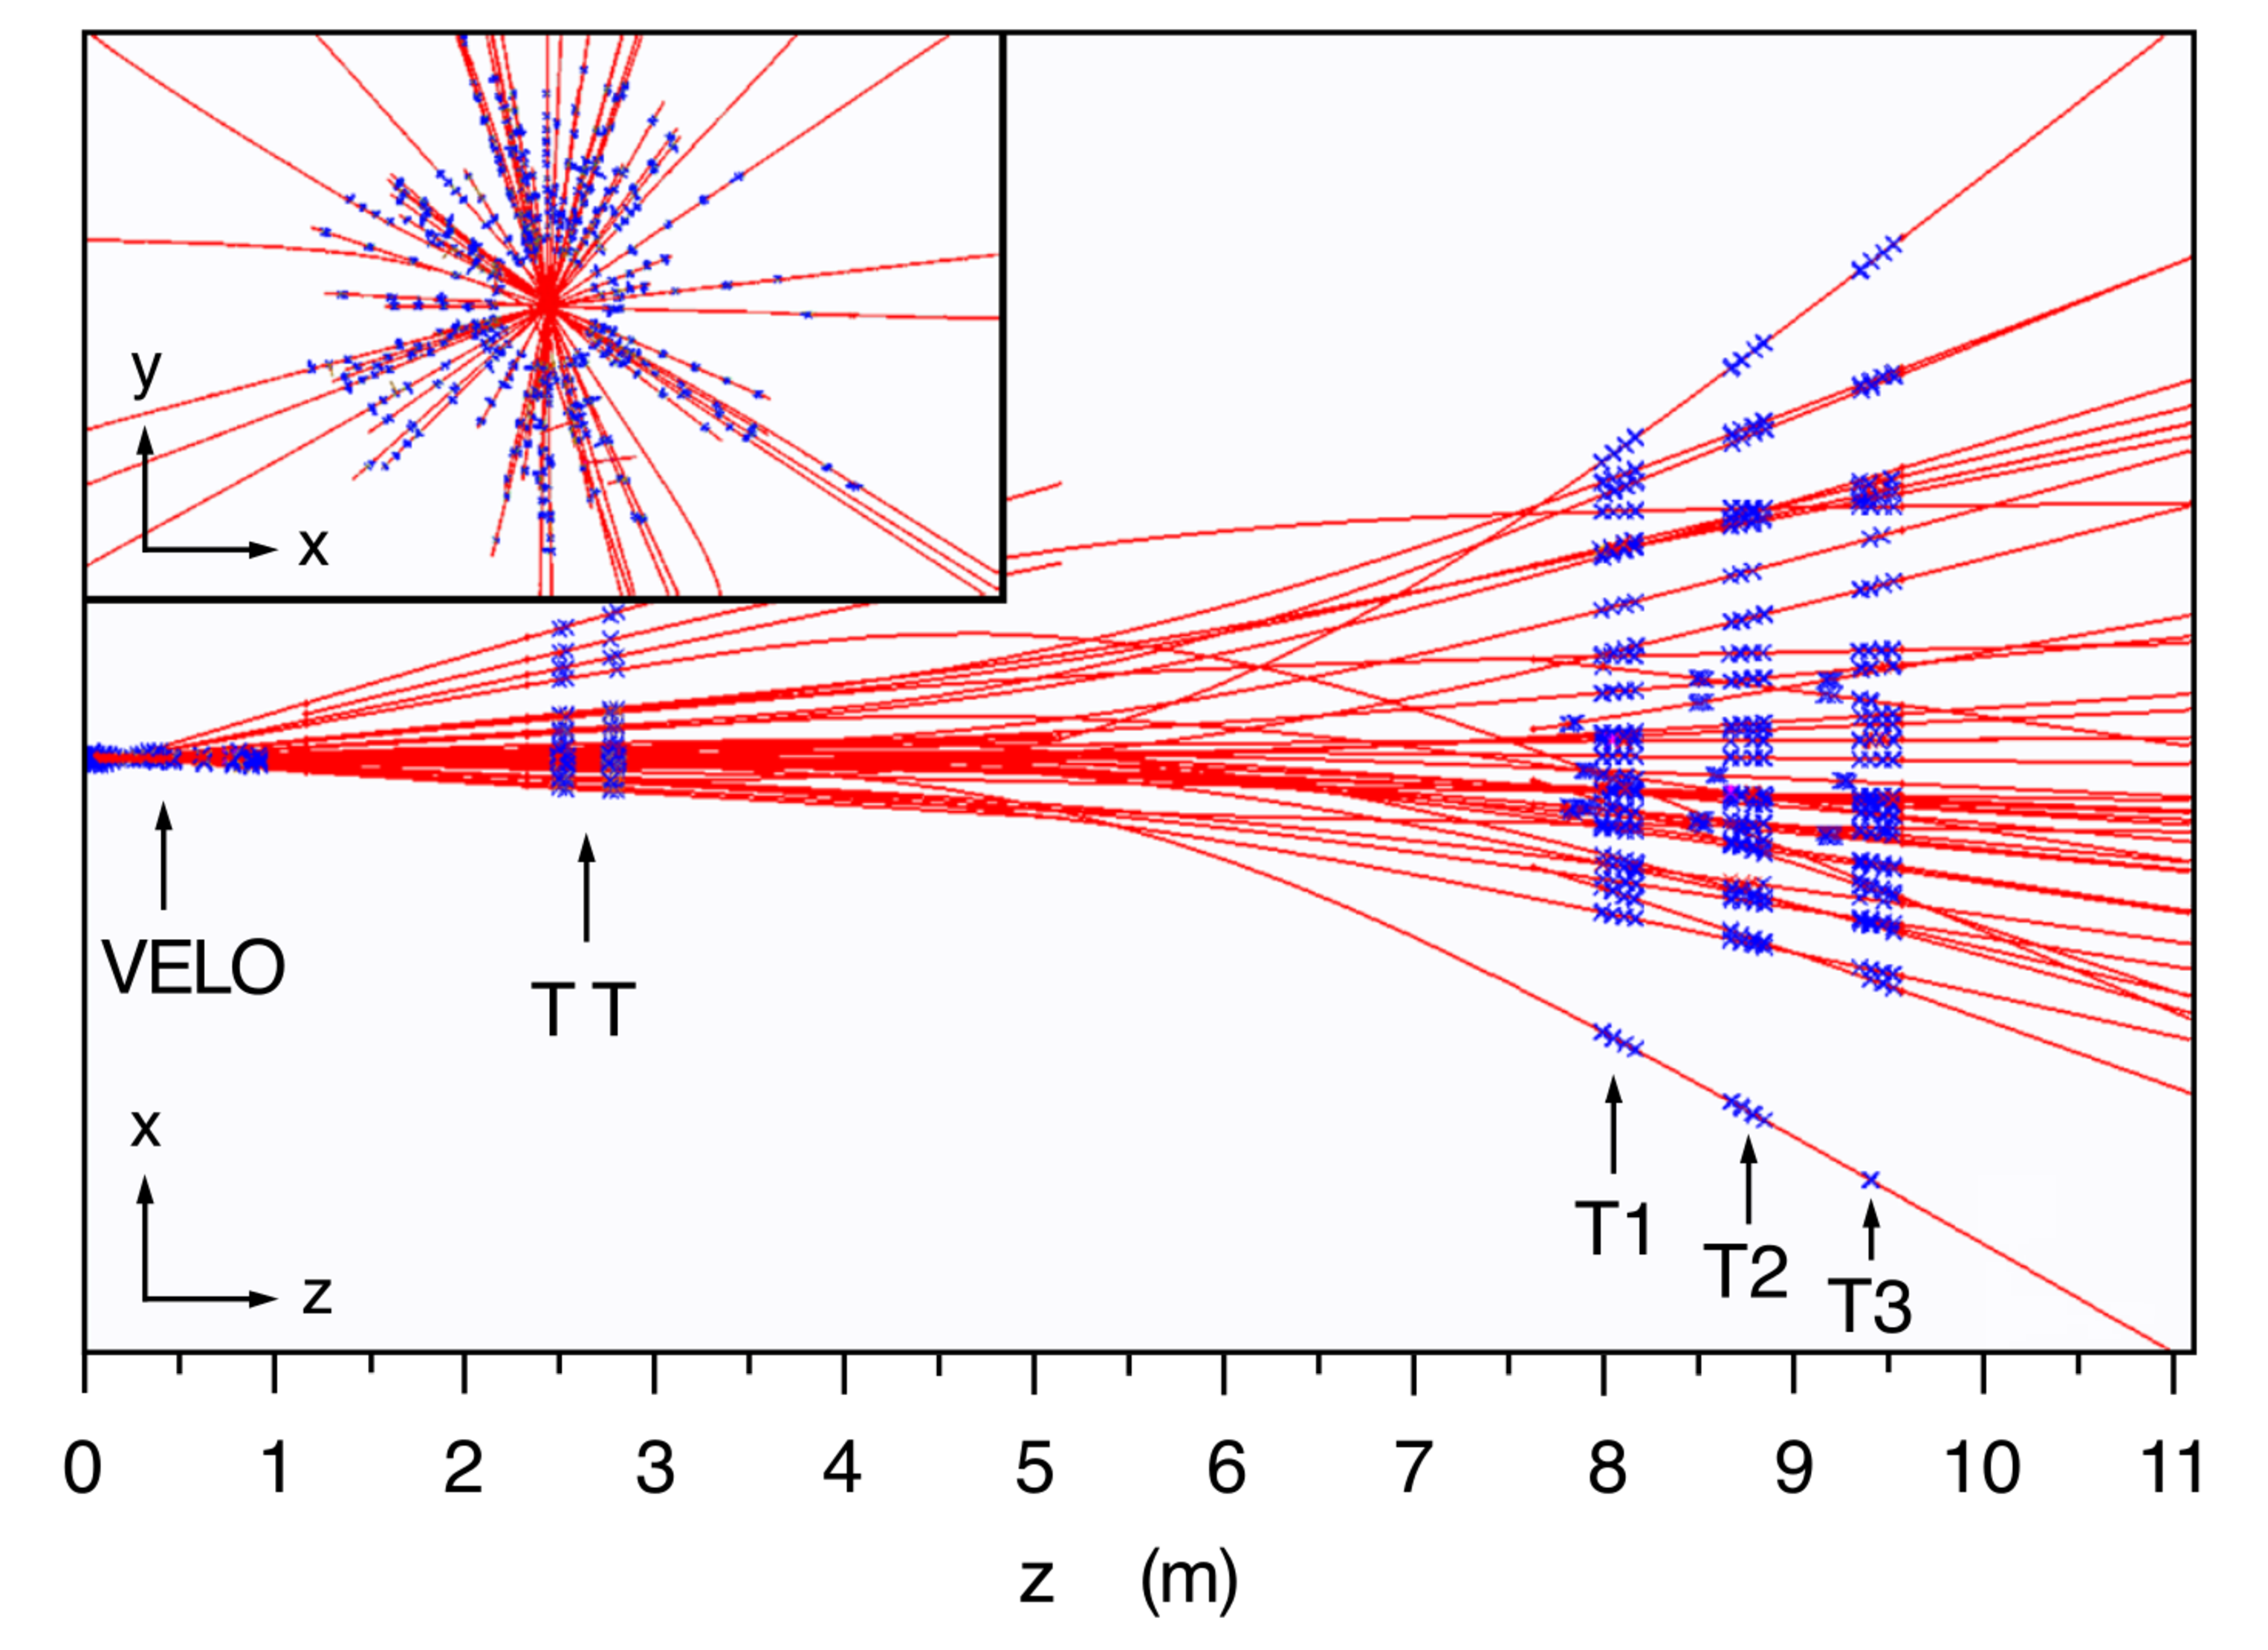
\includegraphics[width=0.7\linewidth]{figures/detector/tracking.pdf}
\caption{Display of the reconstructed tracks (red) and assigned hits (blue) in an event in the $x-z$ plane. The insert shows a zoom into the \velo region in the $x-y$ plane. Reproduced from Ref \cite{LHCb-DP-2014-002}.}
\label{tracking}
\end{figure}

The TT and IT are constructed from silicon microstrip detectors, arranged as shown in \fig\ref{itandot}. The TT is a planar detector 150\cm wide and 130\cm high, located upstream of the dipole magnet, covering the full detector acceptance. At the centre of each of the three T-stations downstream of the magnet, the IT is arranged in a cross shape, 120~\cm wide and 40~\cm high, around the beam pipe. Each of the four planar tracking stations are composed of four layers of modules with the first and fourth layers mounted vertically and the second and third layers mounted at $+5^{\circ}$ and $-5^{\circ}$ from the vertical, respectively. The TT has an active area of 8.4\ma and the IT has an active area of 4.0\ma, and both use silicon microstrip sensors with a strip pitch of about
200\mum, giving a single hit resolution of around 50\mum.

The OT is a straw drift tube detector for the tracking of charged particles and the measurement of their momentum over the full detector acceptance. The straw tubes in each station are arranged in four modules, with the same rotation of modules as in the TT and IT. Each module contains two staggered layers of drift-tubes. The total active area is approximately 6$\times$5~\mma and contains approximately 55,000 single straw-tube channels, with inner diameters of 4.9~\mm. The straw tubes are filled with a gas mixture containing 70\% argon and 30\% carbon dioxide, which guarantees a drift time below 50~\ns and sufficient drift-coordinate resolution of 200~\mum.

\begin{figure}
\centering
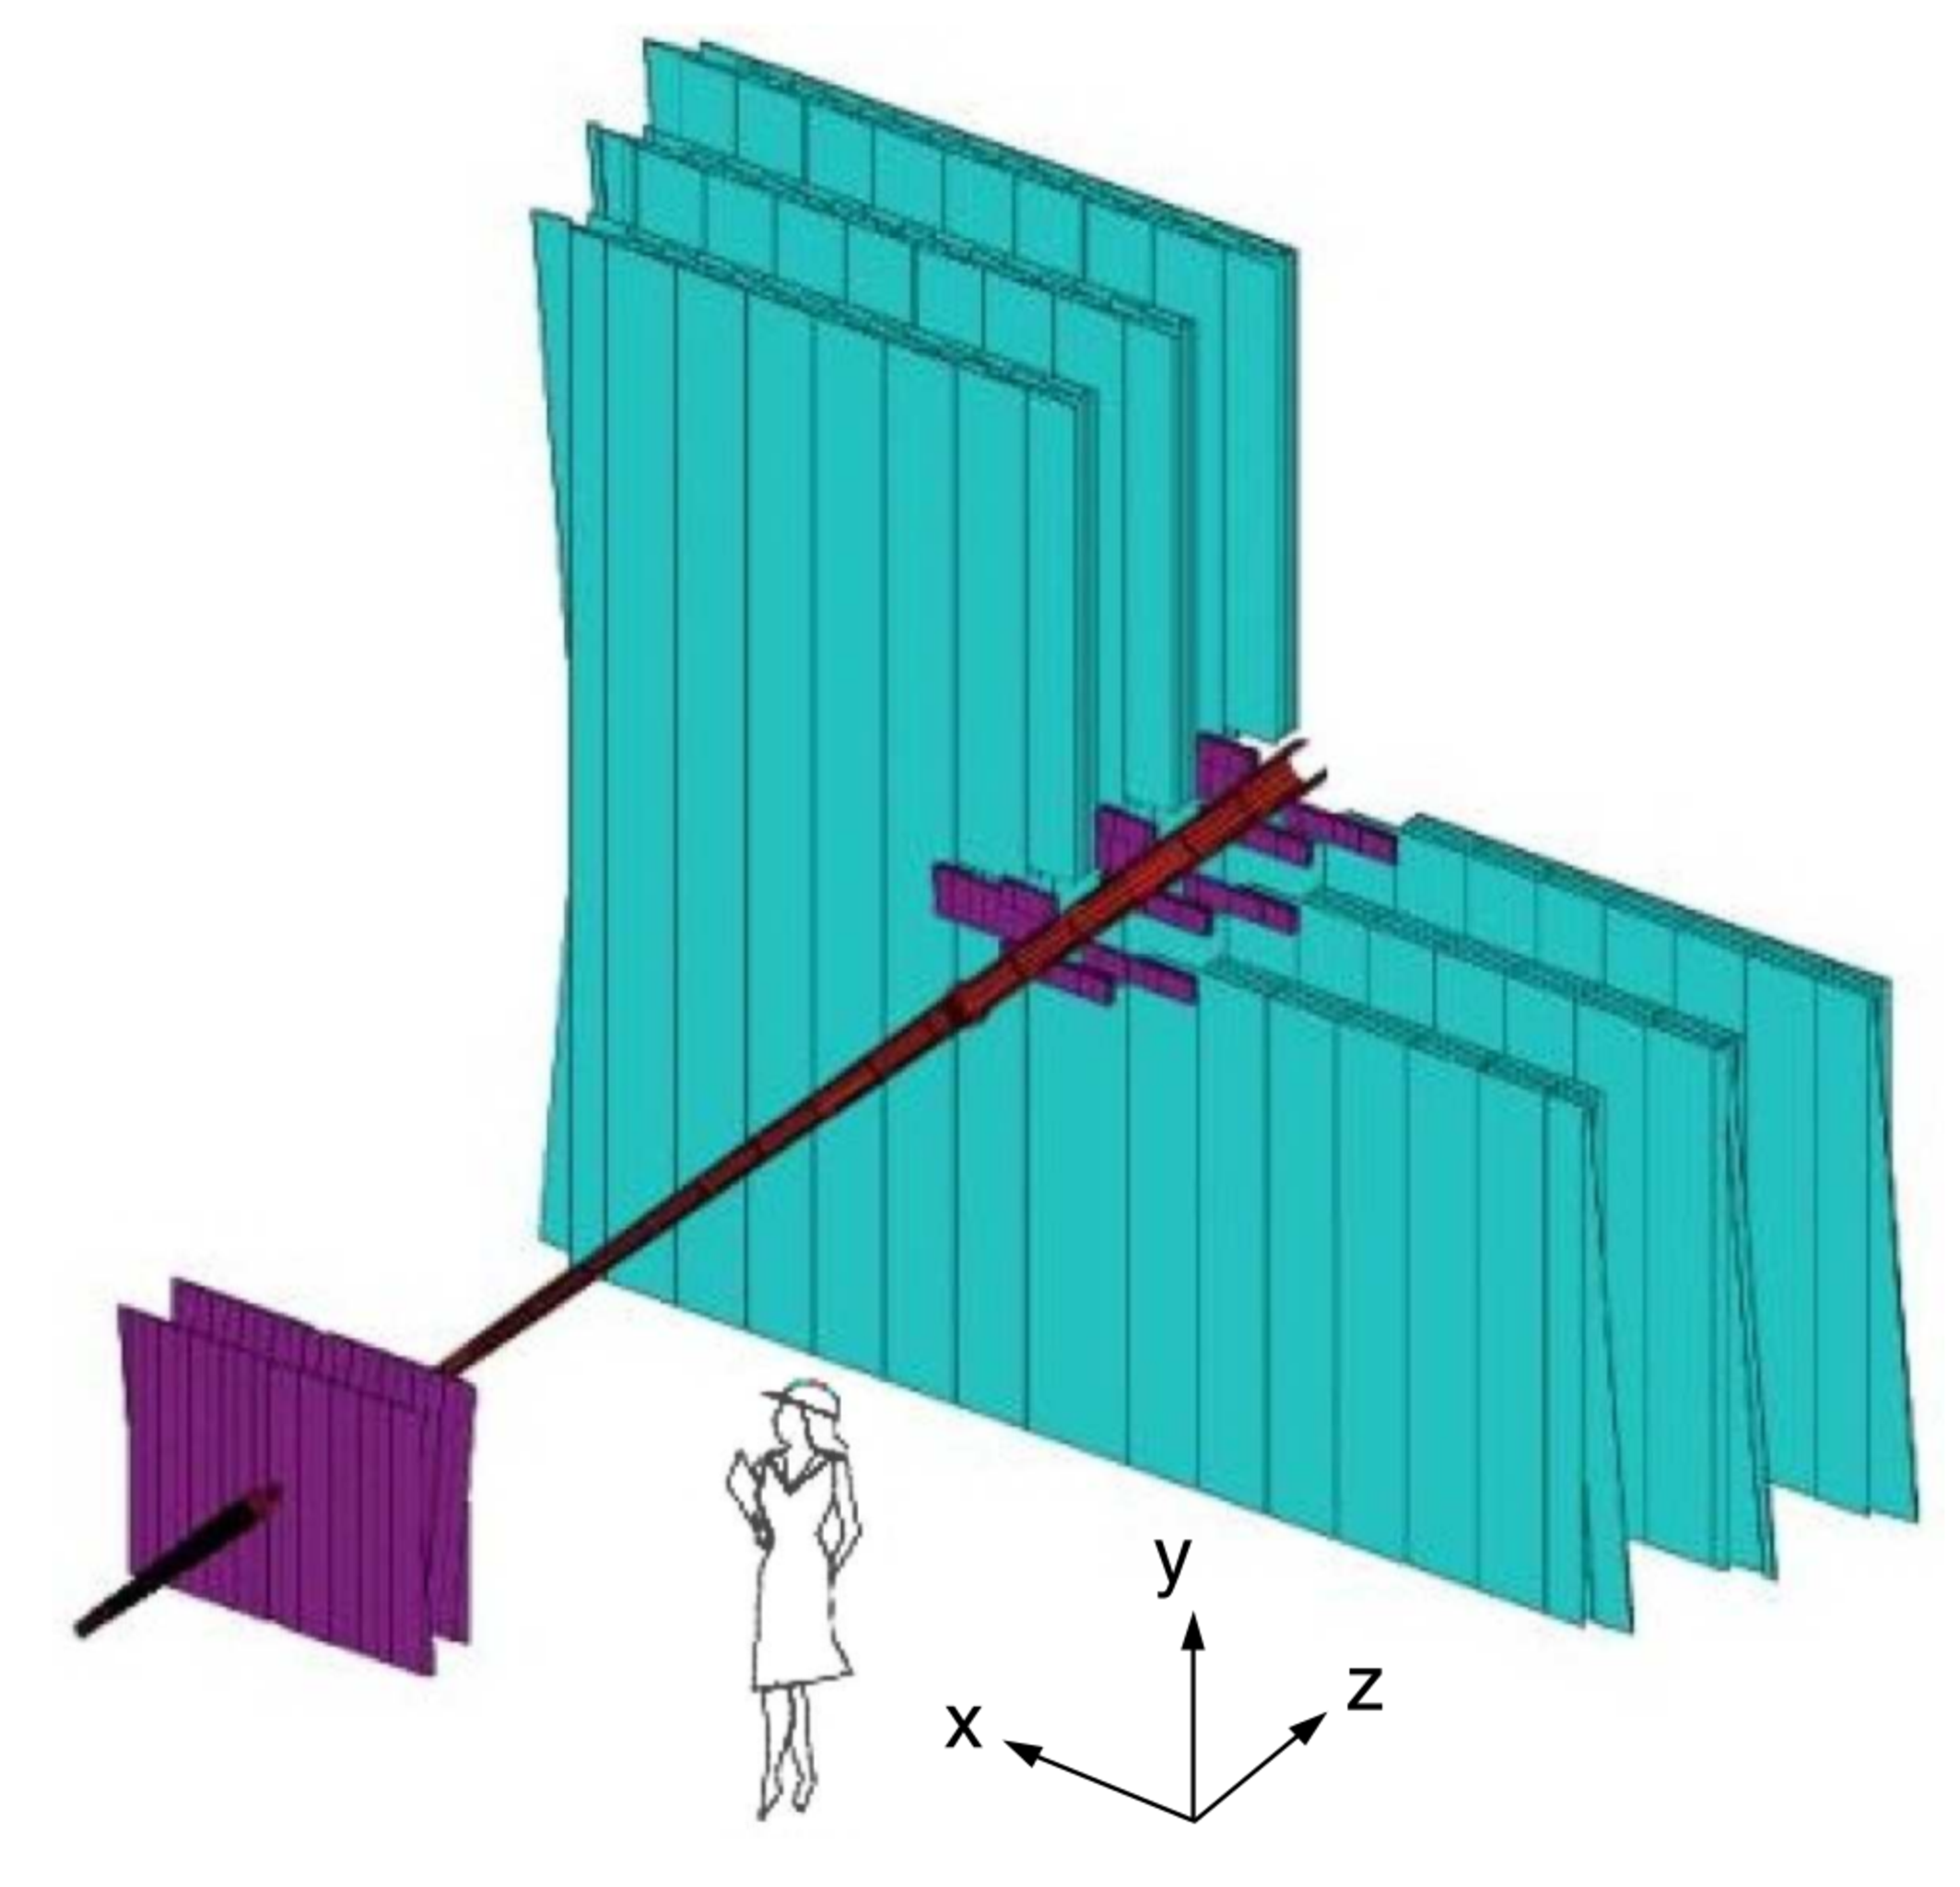
\includegraphics[width=0.5\linewidth]{figures/detector/InnerAndOuterTracker.pdf}
\caption{Arrangement of the layers of the IT and OT. Reproduced from Ref.~\cite{lhcbdetector2008}.}
\label{itandot}
\end{figure}

The dipole magnet, with an integrated magnetic field of about 4~Tm, enables the momentum of charged particles to be measured by bending the trajectory of charged particles in the horizontal plane. In order to achieve the required momentum resolution, the integrated magnetic field, $B = \int{\mathcal{B} dl}$, is measured to a precision corresponding to $\delta B /B \sim 10^{-4}$, where $\mathcal{B}$ is the magnetic field density. Since positively and negatively charged particles will bend in opposite directions, a charge detection asymmetry can result if the left and right halves of the detector have different tracking efficiencies. This would affect CP violation studies, such as the one described in this thesis, which involve the measurements of charge asymmetries. Hence, to minimise systematics, the magnetic field direction is reversed regularly during data-taking.

The tracking efficiency is defined as the probability that the trajectory of a charged particle that passes through the full tracking system is reconstructed. The measured tracking efficiency as a function of momentum and pseudorapidity is shown in \fig\ref{trackingeff}. The average efficiency is above 96\% over the momentum range 5 - 200~\gevc and pseudorapidity range, 2 $< \eta <$ 5. \Fig\ref{momentumres} shows the momentum resolution of reconstructed tracks, which is about 0.5\% for particles below 20~\gevc, rising to about 0.8\% for particles around 100 \gevc. 
%In \runone, the efficiency of the OT to detect a hit in the central half of the straw is estimated to be 99.2\%, and the position resolution is determined to be approximately 200~\mum~\cite{LHCb-DP-2013-003}. 

\begin{figure}
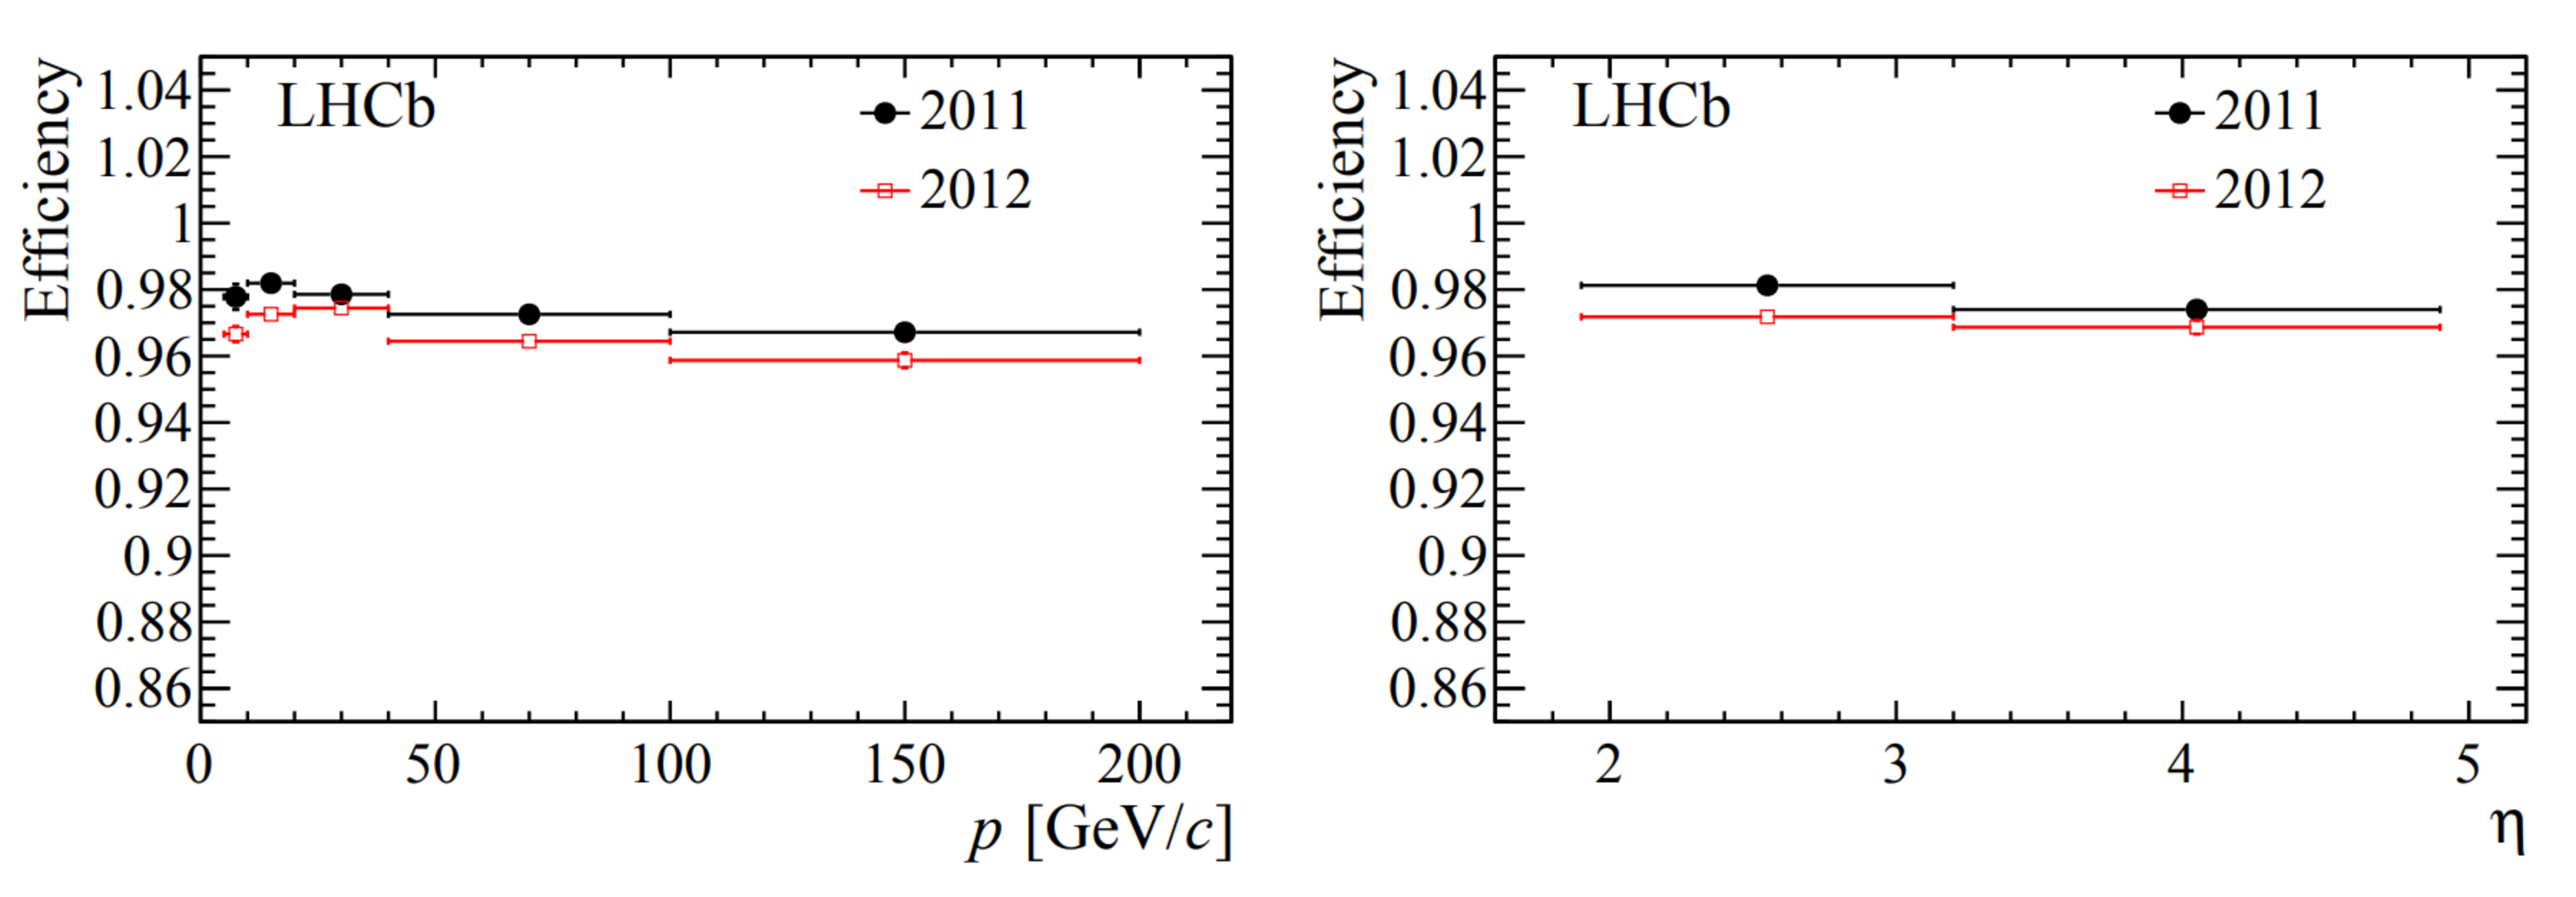
\includegraphics[width=\linewidth]{figures/detector/trackingefficiency.pdf}
\caption{Tracking efficiency as a function of momentum, $p$, and pseudorapidity, $\eta$. The error bars indicate the statistical uncertainty. Reproduced from Ref.~\cite{LHCb-DP-2013-002}.}
\label{trackingeff}
\end{figure}

\begin{figure}
\centering
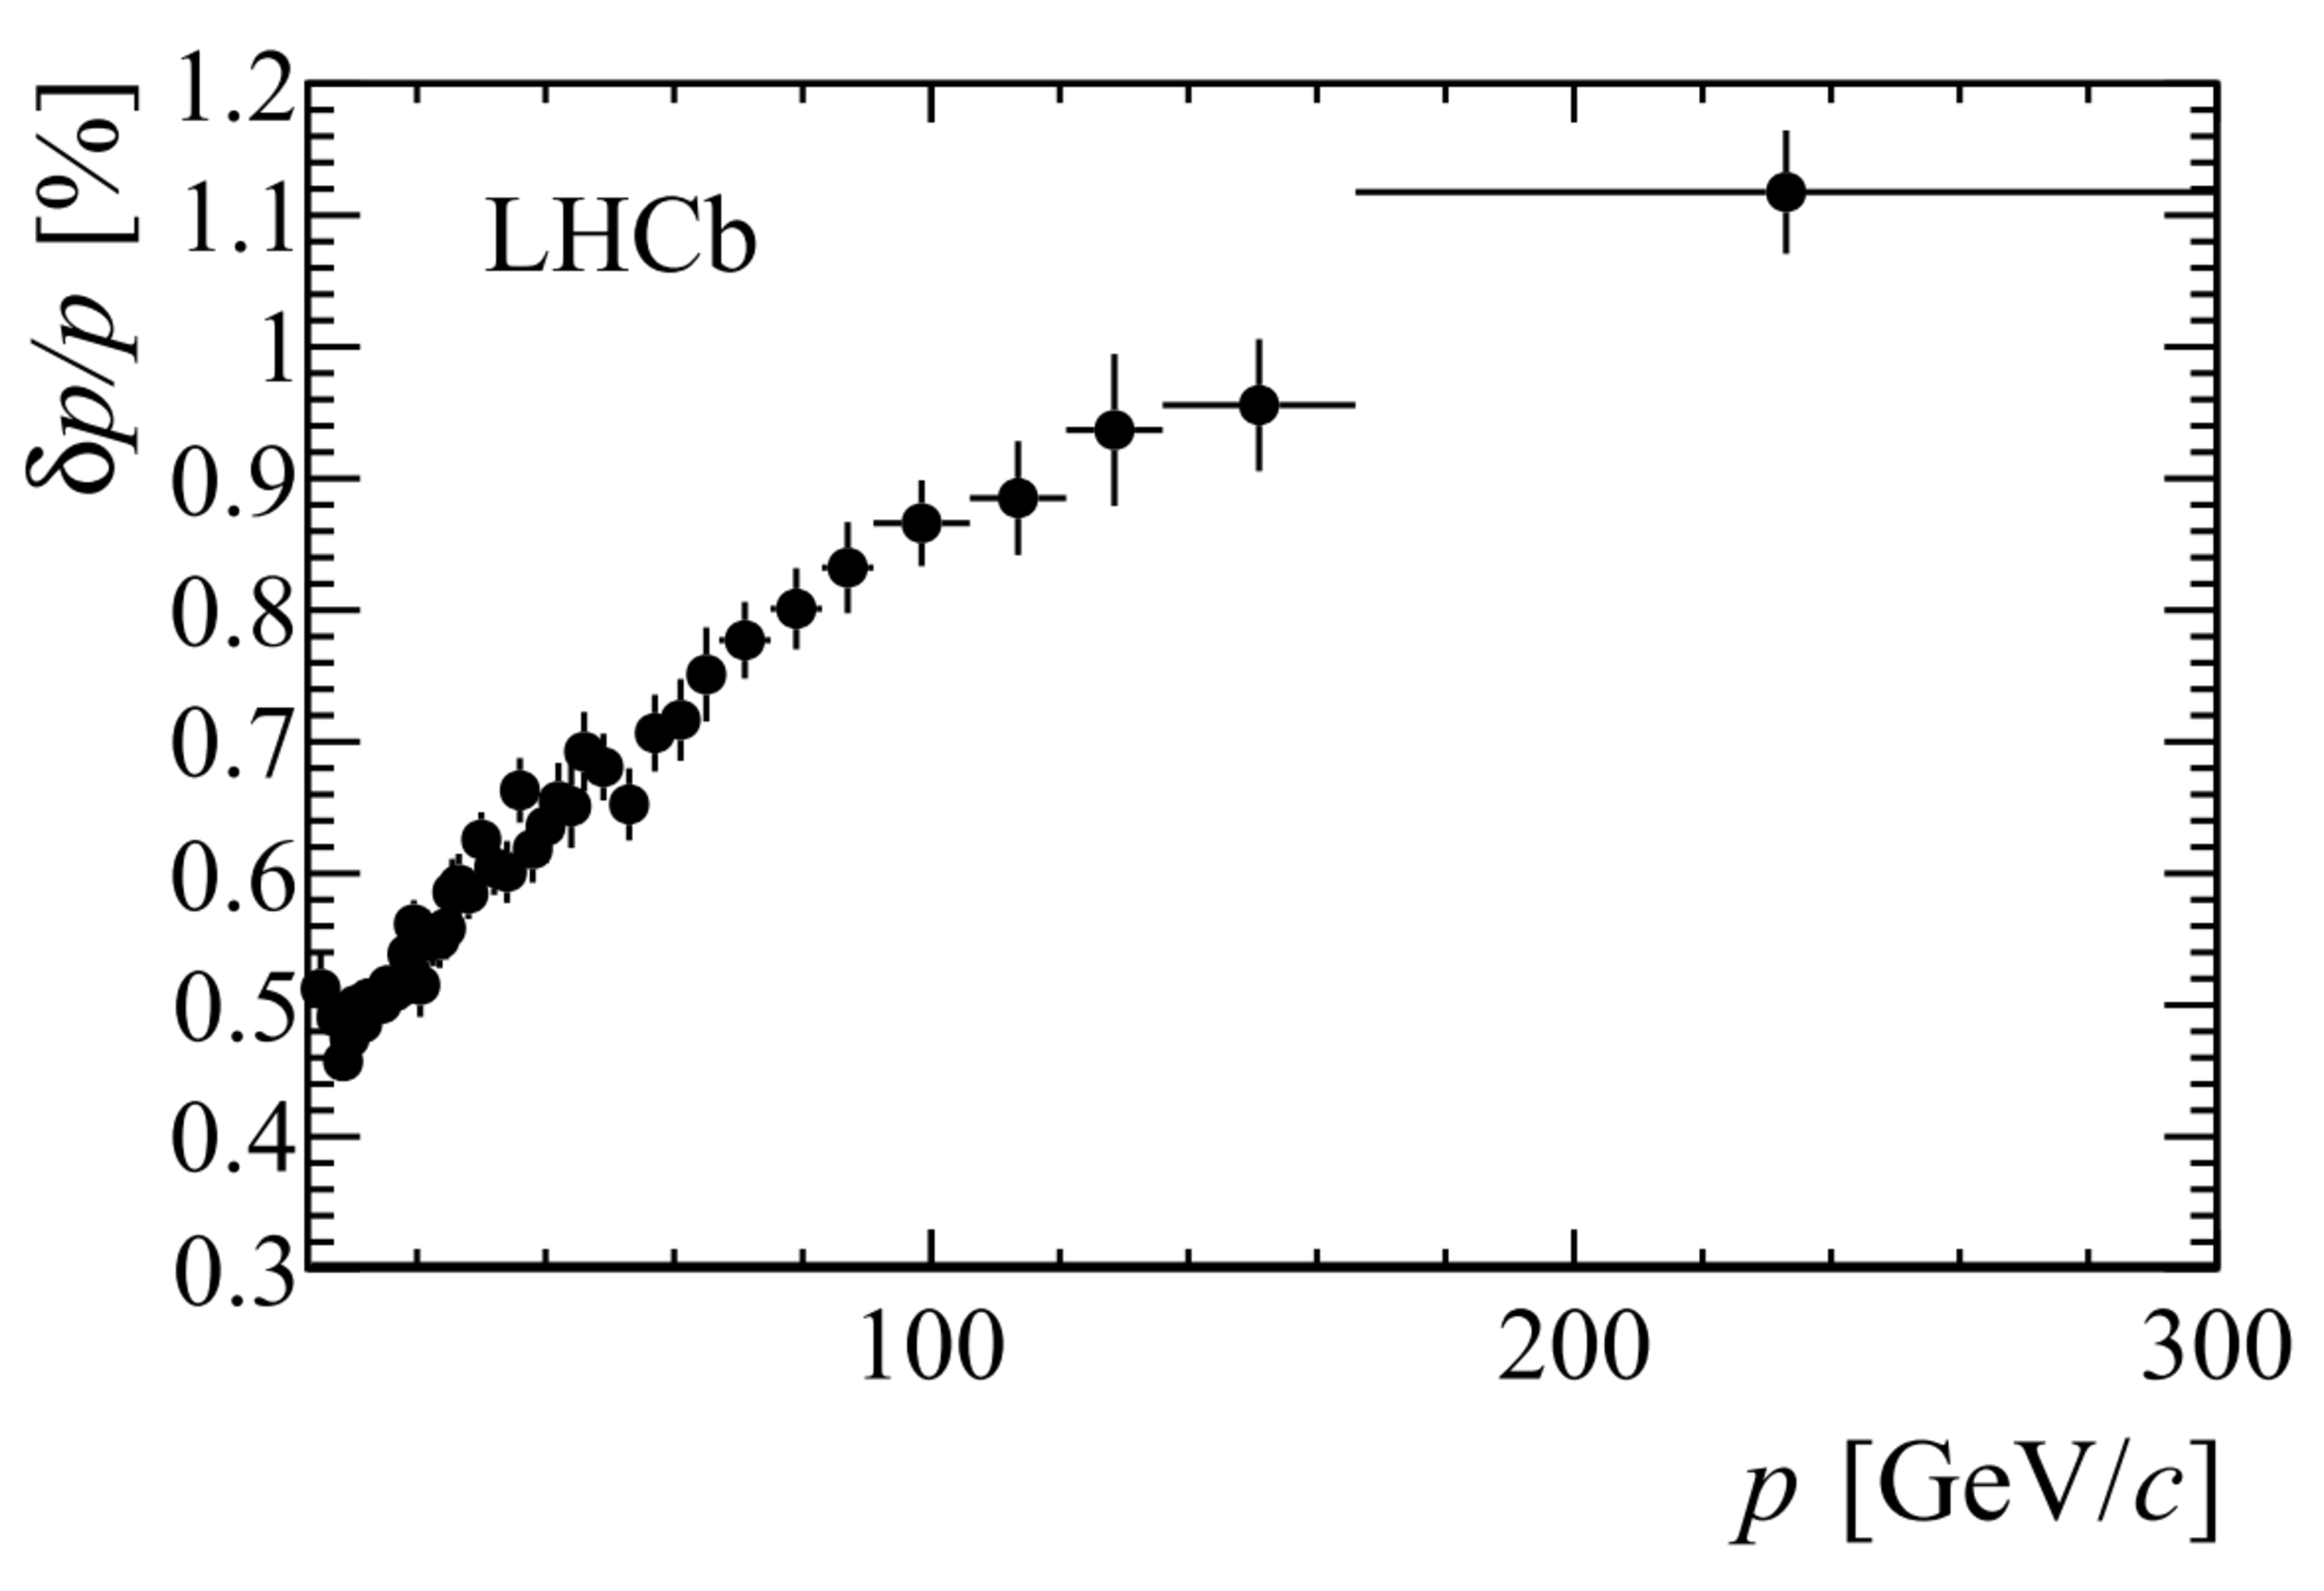
\includegraphics[width=0.5\linewidth]{figures/detector/momentumresolution.pdf}
\caption{Momentum resolution as a function of momentum for tracks that have traversed the entire tracking system. Reproduced from Ref \cite{LHCb-DP-2014-002}.}
\label{momentumres}
\end{figure}
	
\section{The \rich detectors}
\label{sec:detector:rich}

The \rich detectors (RICH 1 and RICH 2)~\cite{LHCb-DP-2012-003} are required for the identification of charged hadrons, specifically pions, kaons and protons. The decay modes of \bquark- and \cquark-flavoured hadrons involve hadronic multibody final states, therefore good particle identification of hadrons over the momentum range 2 - 100 \gevc is vital for reducing the combinatorial backgrounds. The RICH detectors utilise the idea that Cherenkov radiation is produced whenever a charged particle of velocity $v$, travelling through a dielectric medium of refractive index $n$, exceeds the speed of light in that medium, $c/n$. The particle produces a cone of light with an opening angle of $\theta_{CK}$ relative to the direction of the particle's propagation, given by
\begin{equation}
\cos\left(\theta_{CK}\right) = \frac{1}{n\beta} \text{ ,     where }  \beta = v/c \text{ .}
\label{cherenkov}
\end{equation}
By measuring $\theta_{CK}$ using the \rich detectors and the momentum from the magnet and tracking systems, a mass hypothesis can be determined, which provides discrimination between particle species. The relationship between Cherenkov angle and momentum for different particle species is shown in \fig\ref{richseparation}. It can be seen that the separation tends to zero as the momentum increases, as expected from \eqn\ref{cherenkov}, since as $\beta \rightarrow 1$, the Cherenkov angle becomes independent of particle momentum and mass. For a given dielectric medium, there is a low momentum threshold, defined when $\beta = 1/n$, where below this value of $\beta$ no Cherenkov light is emitted. Discrimination of lower momentum (higher mass) particles is then only possible with a dielectric medium of higher refractive index.

\begin{figure}
\centering
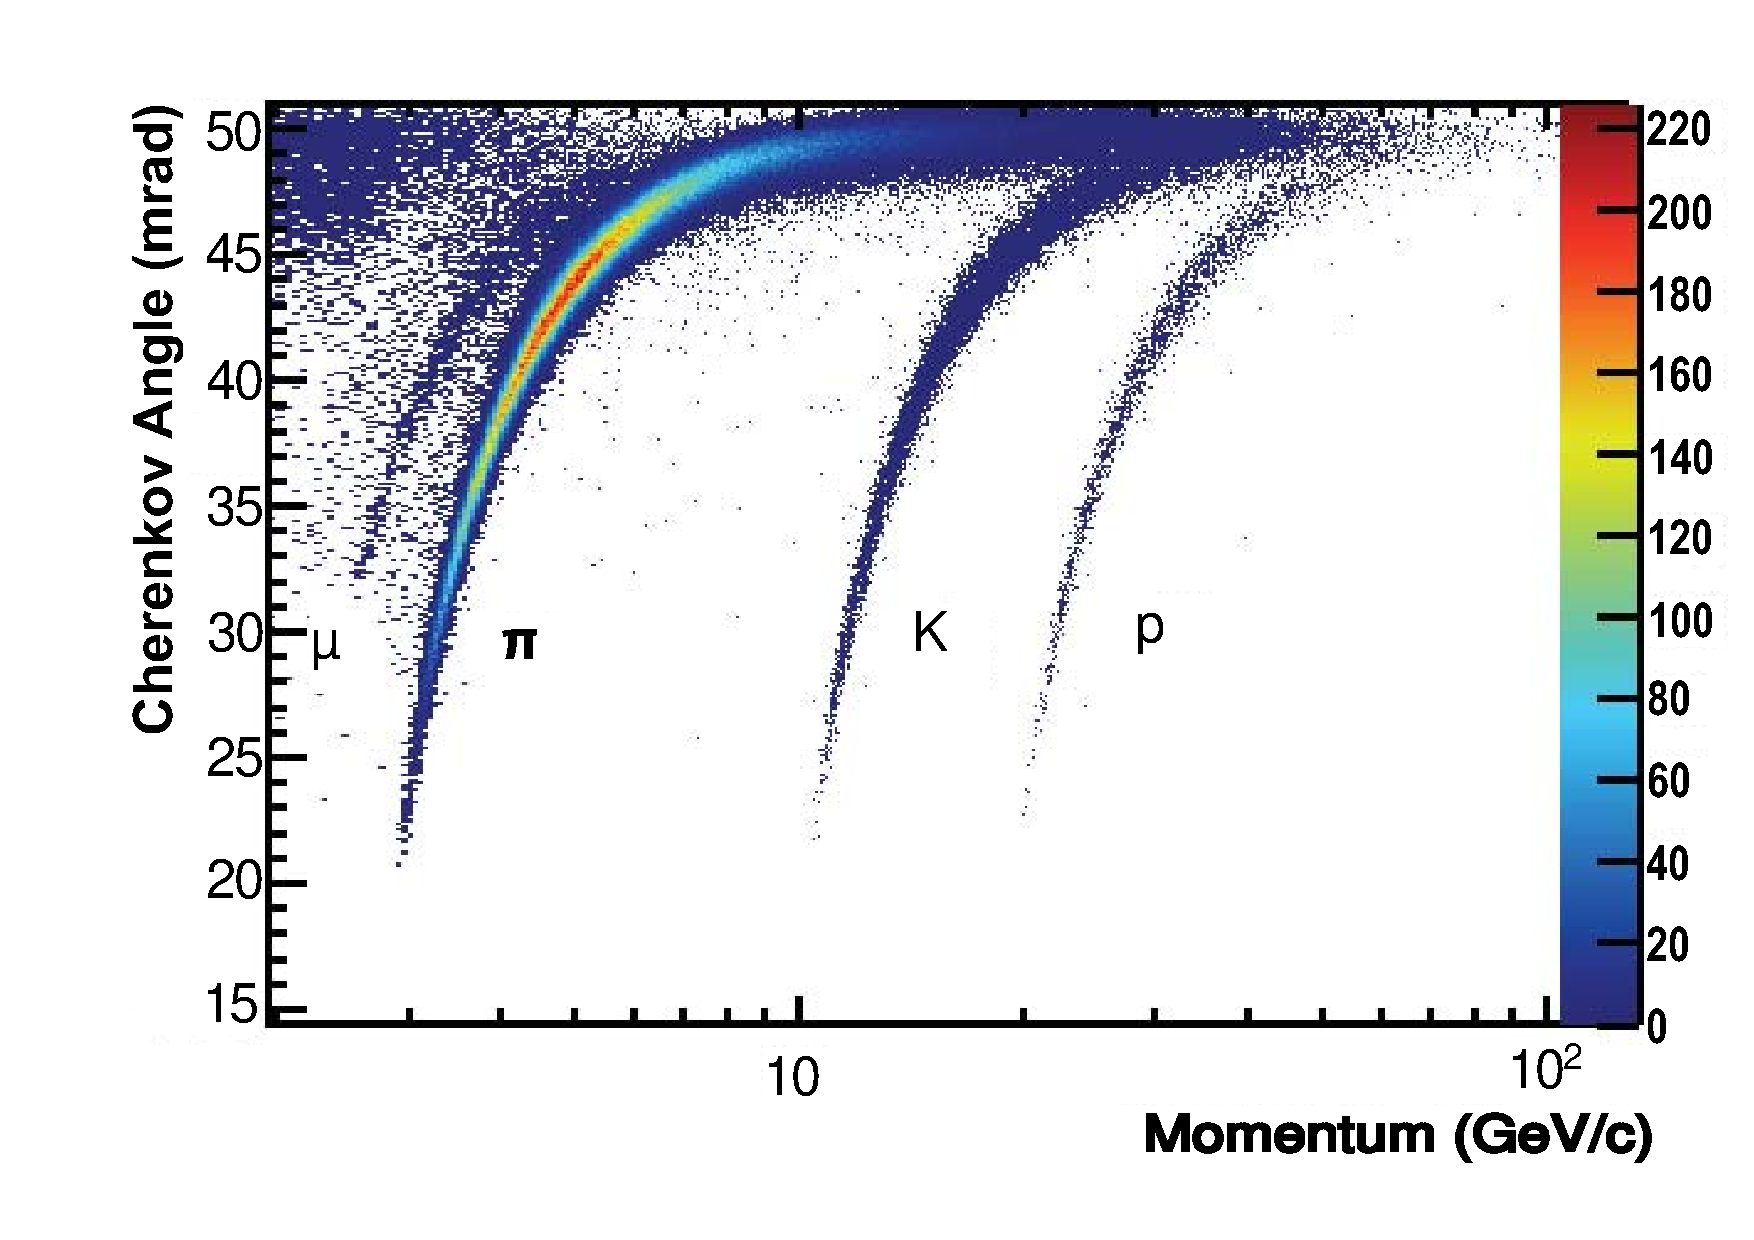
\includegraphics[width=0.8\linewidth]{figures/detector/richseparation.pdf}
\caption{Cherenkov angle measured as a function of momentum in the RICH1 $C_{4}F_{10}$ radiator for isolated tracks. The Cherenkov bands for muons, pions, kaons and protons are clearly visible. Reproduced from Ref \cite{LHCb-DP-2012-003}.}
\label{richseparation}
\end{figure}

Two \rich detectors are used to cover the full \lhcb momentum range; RICH 1 is positioned upstream of the magnet covering the momentum range 2 to 60~\gevc, using two radiators: C$_4$F$_{10}$ ($n = 1.0014$) and Aerogel ($n = 1.03$) in Run 1, although the Aerogel radiator was subsequently removed for Run 2. RICH 2 is located downstream of the magnet and covers the higher momentum range, 15 to 100~\gevc, utilising a CF$_4$ radiator ($n = 1.0005$). While RICH 1 covers the full detector acceptance, RICH 2 covers a limited angular acceptance of $~\sim \pm 15$~mrad to $\pm 120$~mrad in the horizontal direction and $\pm 100$~mrad in the vertical direction. In each RICH detector the cone of Cherenkov radiation that radiates from the charged particle is reflected by spherical focusing primary mirrors and planar secondary mirrors to project a ring onto the focal plane containing an array of Hybrid Photon Detectors (HPDs). The HPDs contain pixels of area $2\times 2$~\mma, which detect the single photons.

One of the main measures of the \rich performance is the resolution of the Cherenkov angle from which the hit positions of the photons can be reconstructed. This is measured from the distribution of the difference between the measured and expected Cherenkov angle for each photon, $\Delta\theta$, given by $\theta_{CK} - \theta_0$, where $\theta_0$ is the expected Cherenkov angle calculated from the momentum of the track and the refractive index of the radiator. \Fig\ref{cherenkov} shows an example of the distributions of $\Delta\theta$, and from these plots the Cherenkov angle resolution is determined to be $(1.618 \pm 0.002)$~mrad for C$_4$F$_{10}$ in RICH1 and $(0.68 \pm 0.02)$~mrad for CF$_4$ in RICH2.

\begin{figure}
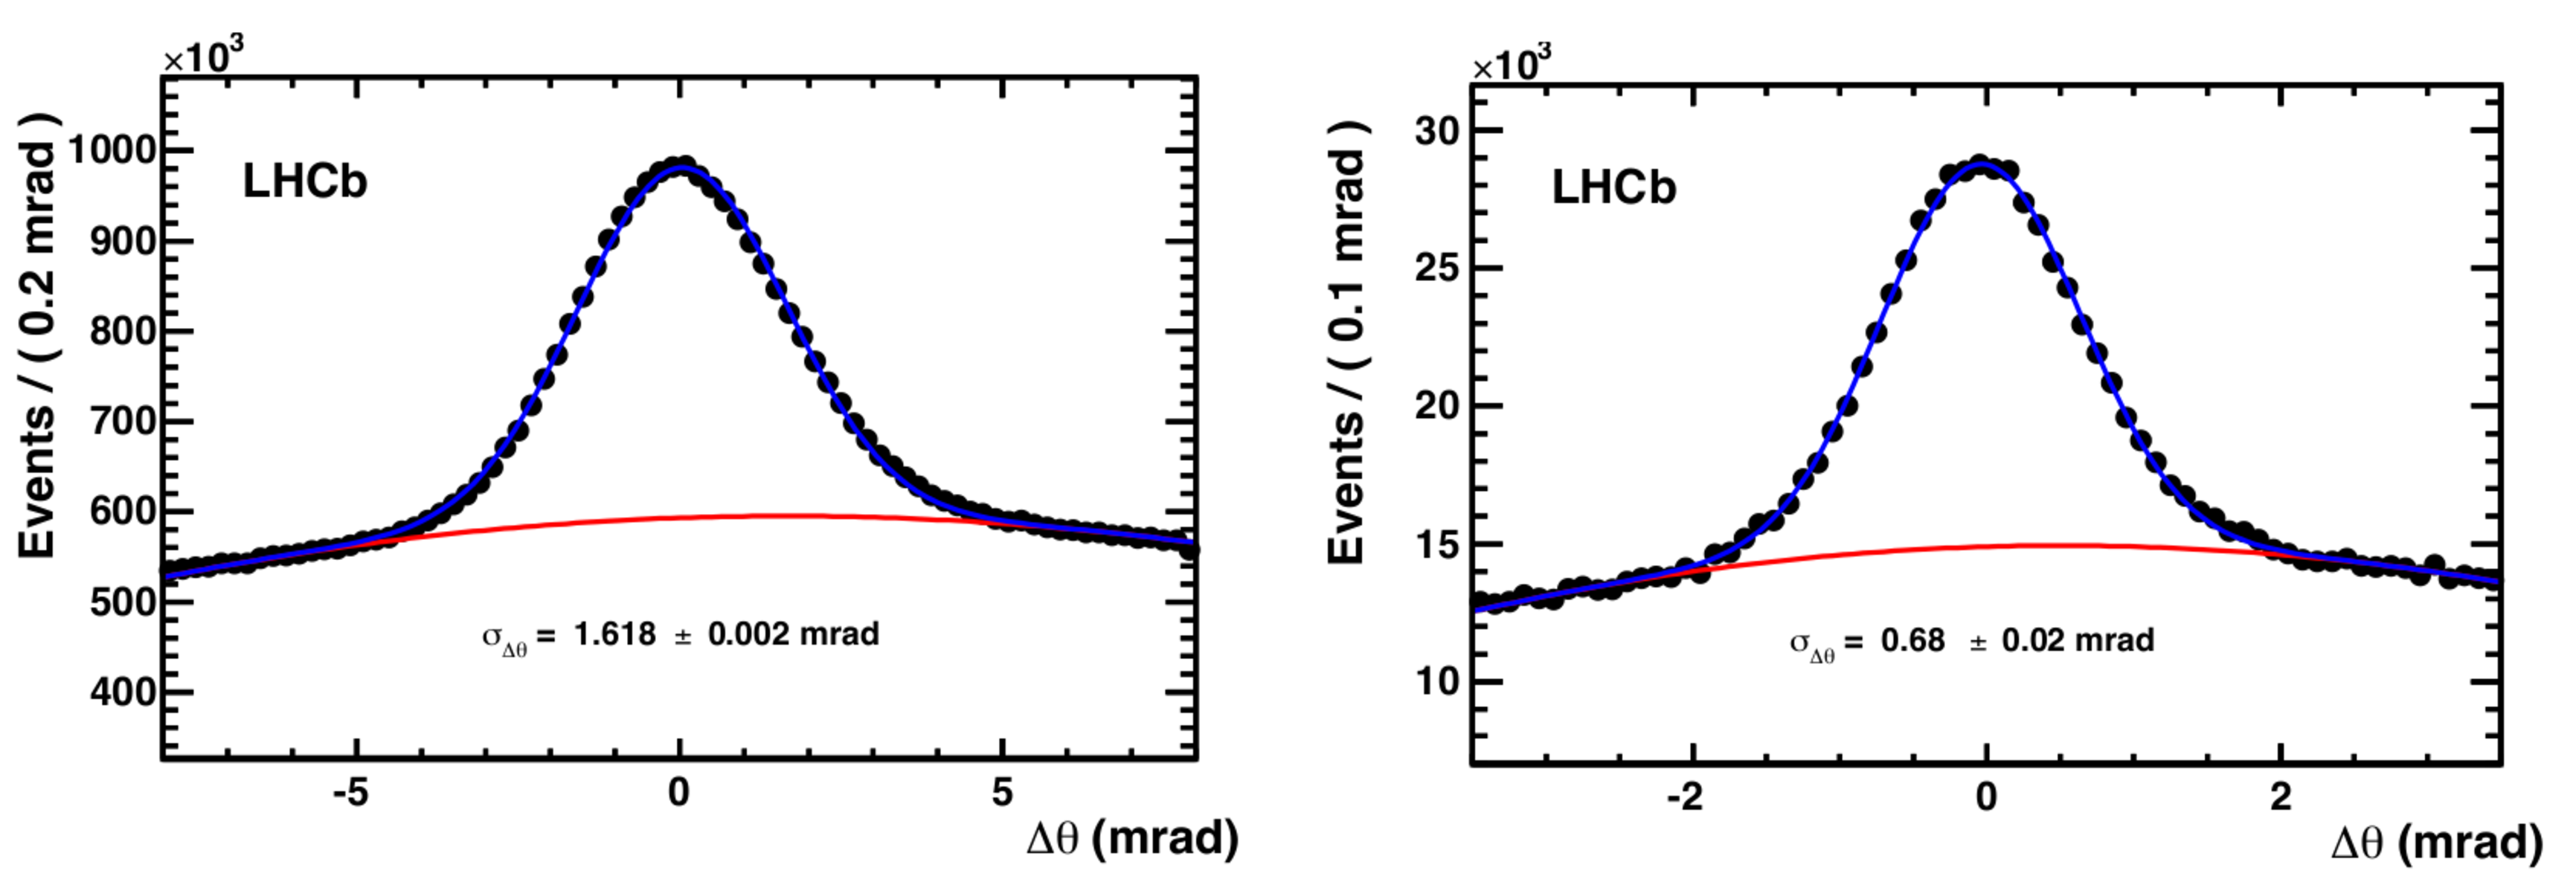
\includegraphics[width=\linewidth]{figures/detector/cherenkov.pdf}
\caption{Cherenkov angle resolution using 2011 data for the RICH 1 gas (left) and RICH 2 gas (right). Reproduced from Ref \cite{LHCb-DP-2012-003}.}
\label{cherenkov}
\end{figure}

Although the RICH system is designed primarily to provide separation between charged hadrons (\pion, $K$ and $p$), it can also provide some information on leptons. Similarly, the calorimeters and muon systems, described below, can provide some hadron identification. A global likelihood hypothesis for each particle type (\pion, $K$, $p$, $e$, $\mu$) is formed by combining the particle likelihood hypotheses as determined by each sub-detector, $\mathcal{L}_X$, for particle hypothesis $X$. Since the most abundant particles from a $pp$ interaction are pions, the pion hypothesis is initially assumed. For each track the differences between a particle hypothesis, $X$, log-likelihood compared to the pion hypothesis is computed:
\begin{equation}
DLLX = \log{\mathcal{L}_X} - \log{\mathcal{L}_{\pi}} \text{ .}
\end{equation}

The PID performance of hadrons can be directly determined from background-free calibration samples of protons, kaons and pions, for example, those produced in \Lz, \Dstarm and \KS decays respectively. The typical kaon PID performance of the \lhcb detector for both \runone and \runtwo is shown in \fig\ref{richperformance}. It can be seen that the overall performance of the \rich system has improved in \runtwo. These improvements from \runone to \runtwo are both due to changes in the running conditions, for example the increase in beam energy and the change in trigger conditions, and the intrinsic performance of the \rich system, mainly from the removal of the aerogel radiator.

\begin{figure}
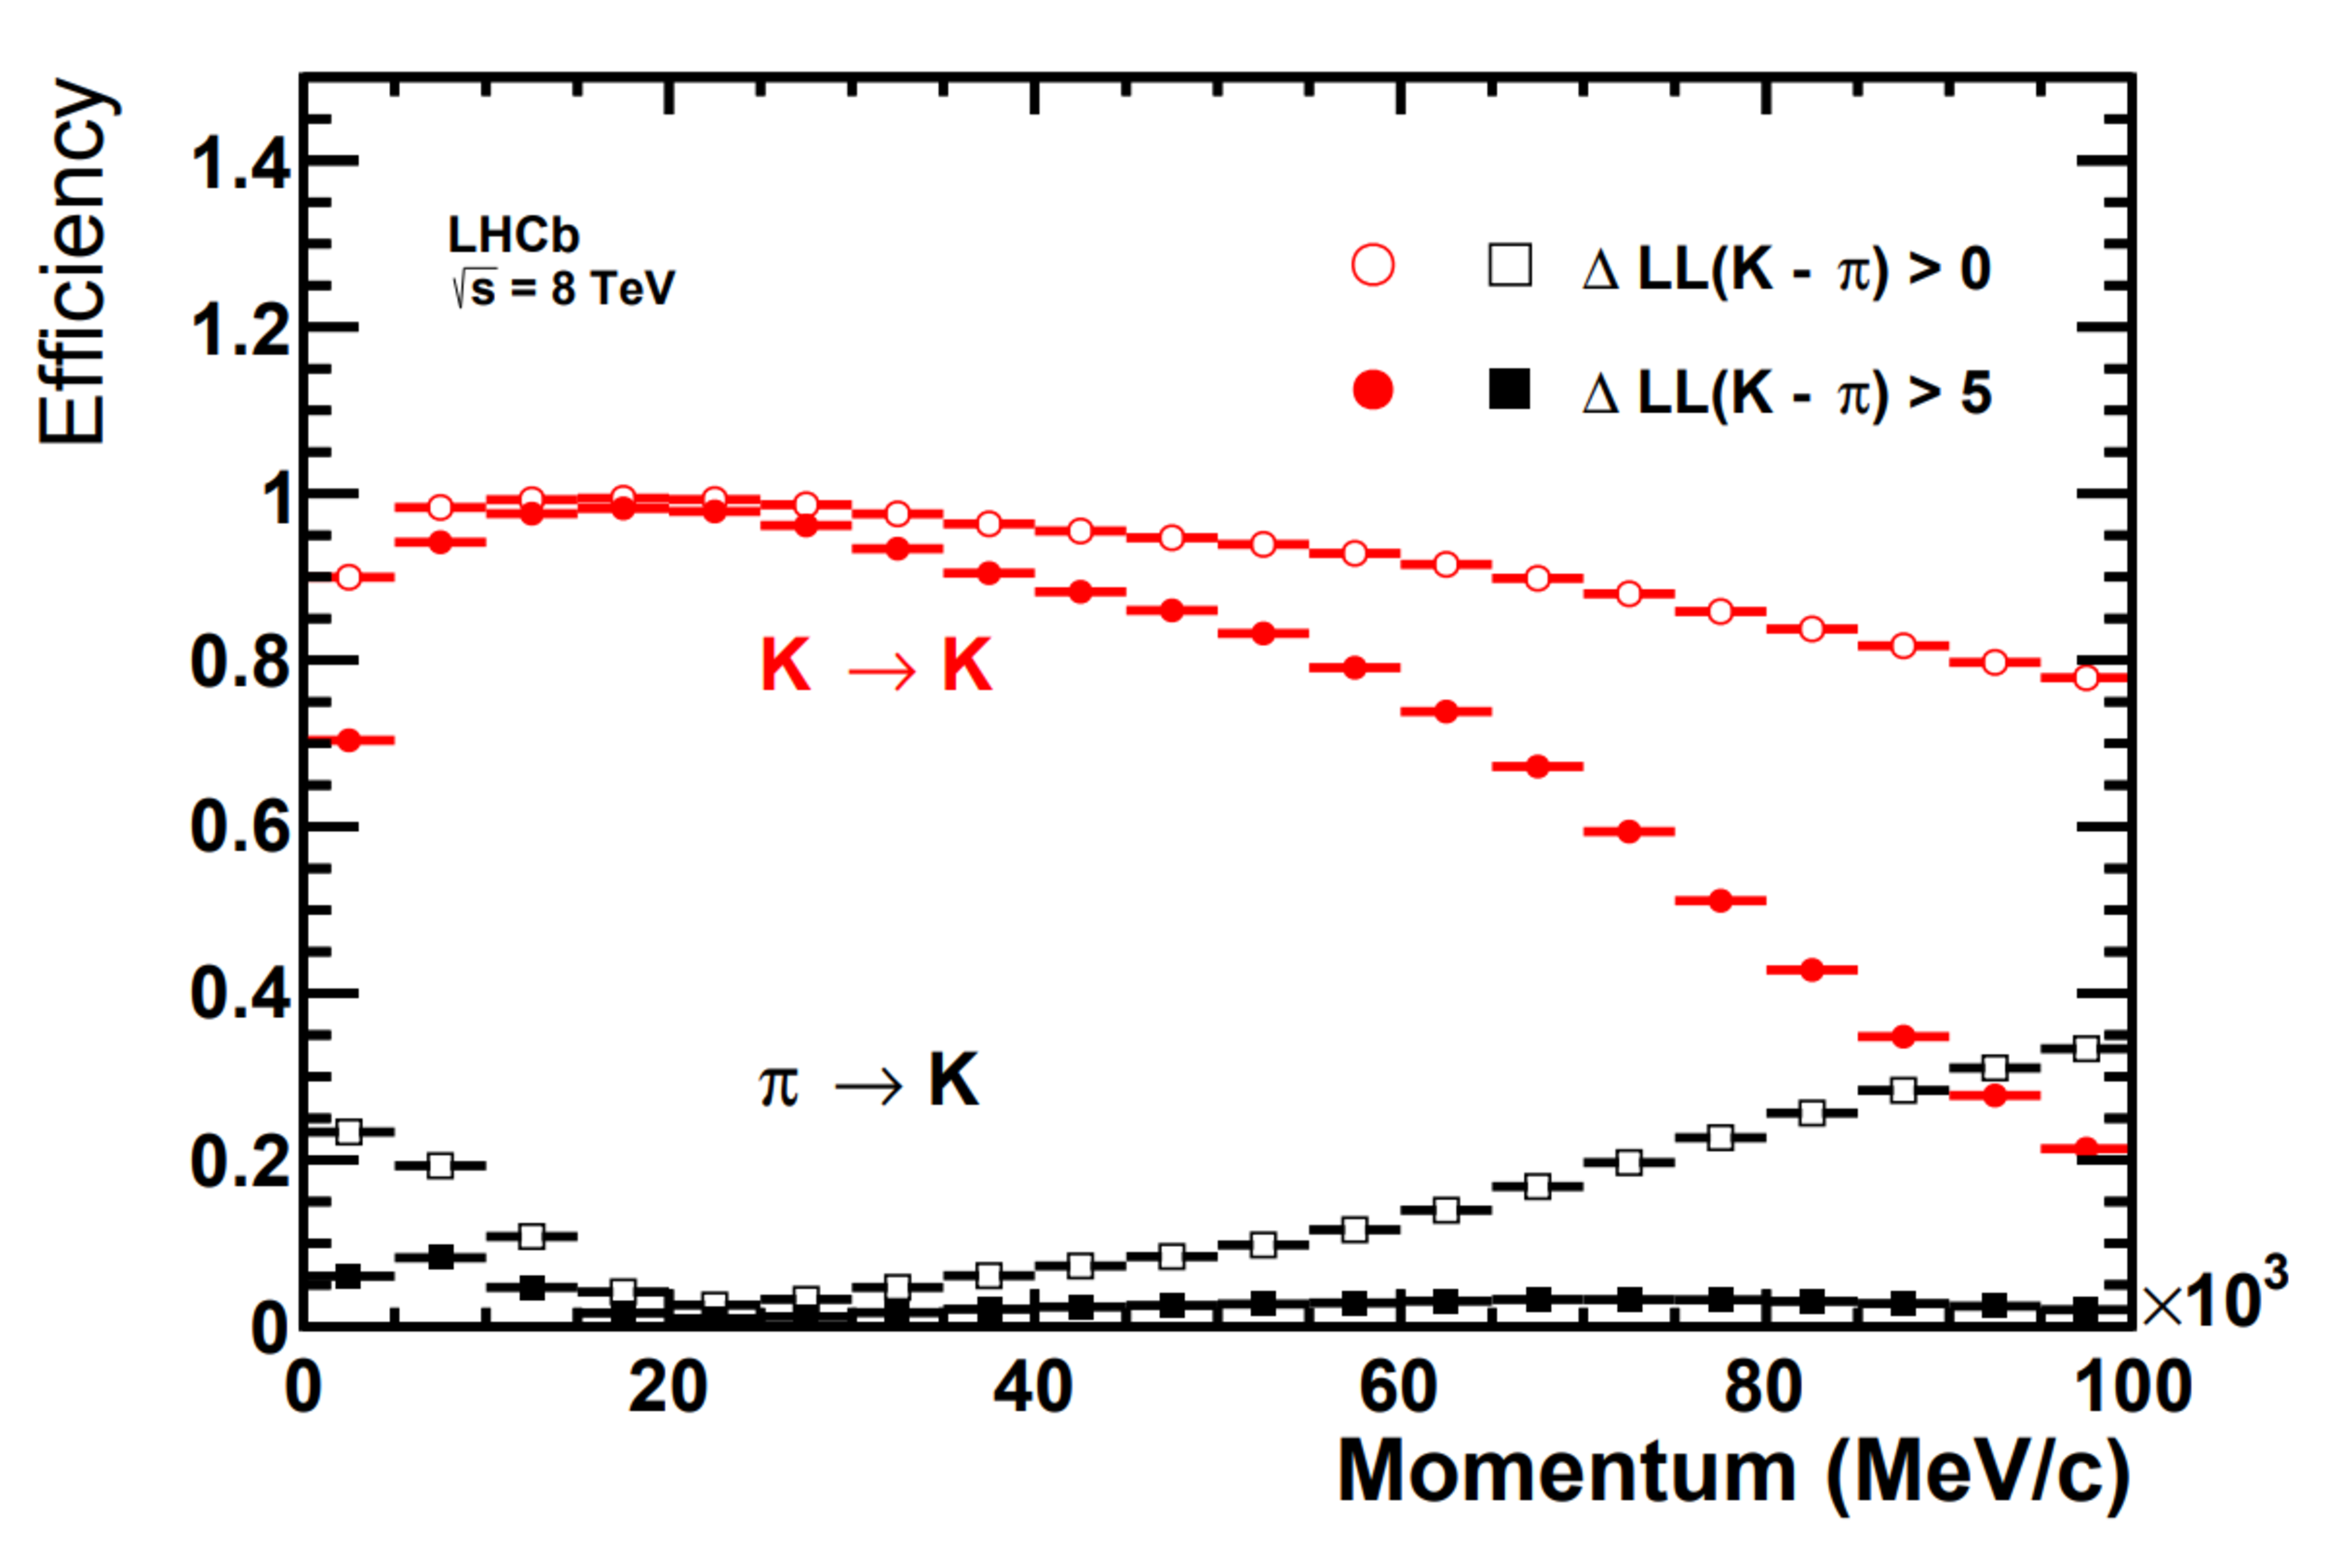
\includegraphics[width=0.5\linewidth]{figures/detector/richperformance_run1.pdf}
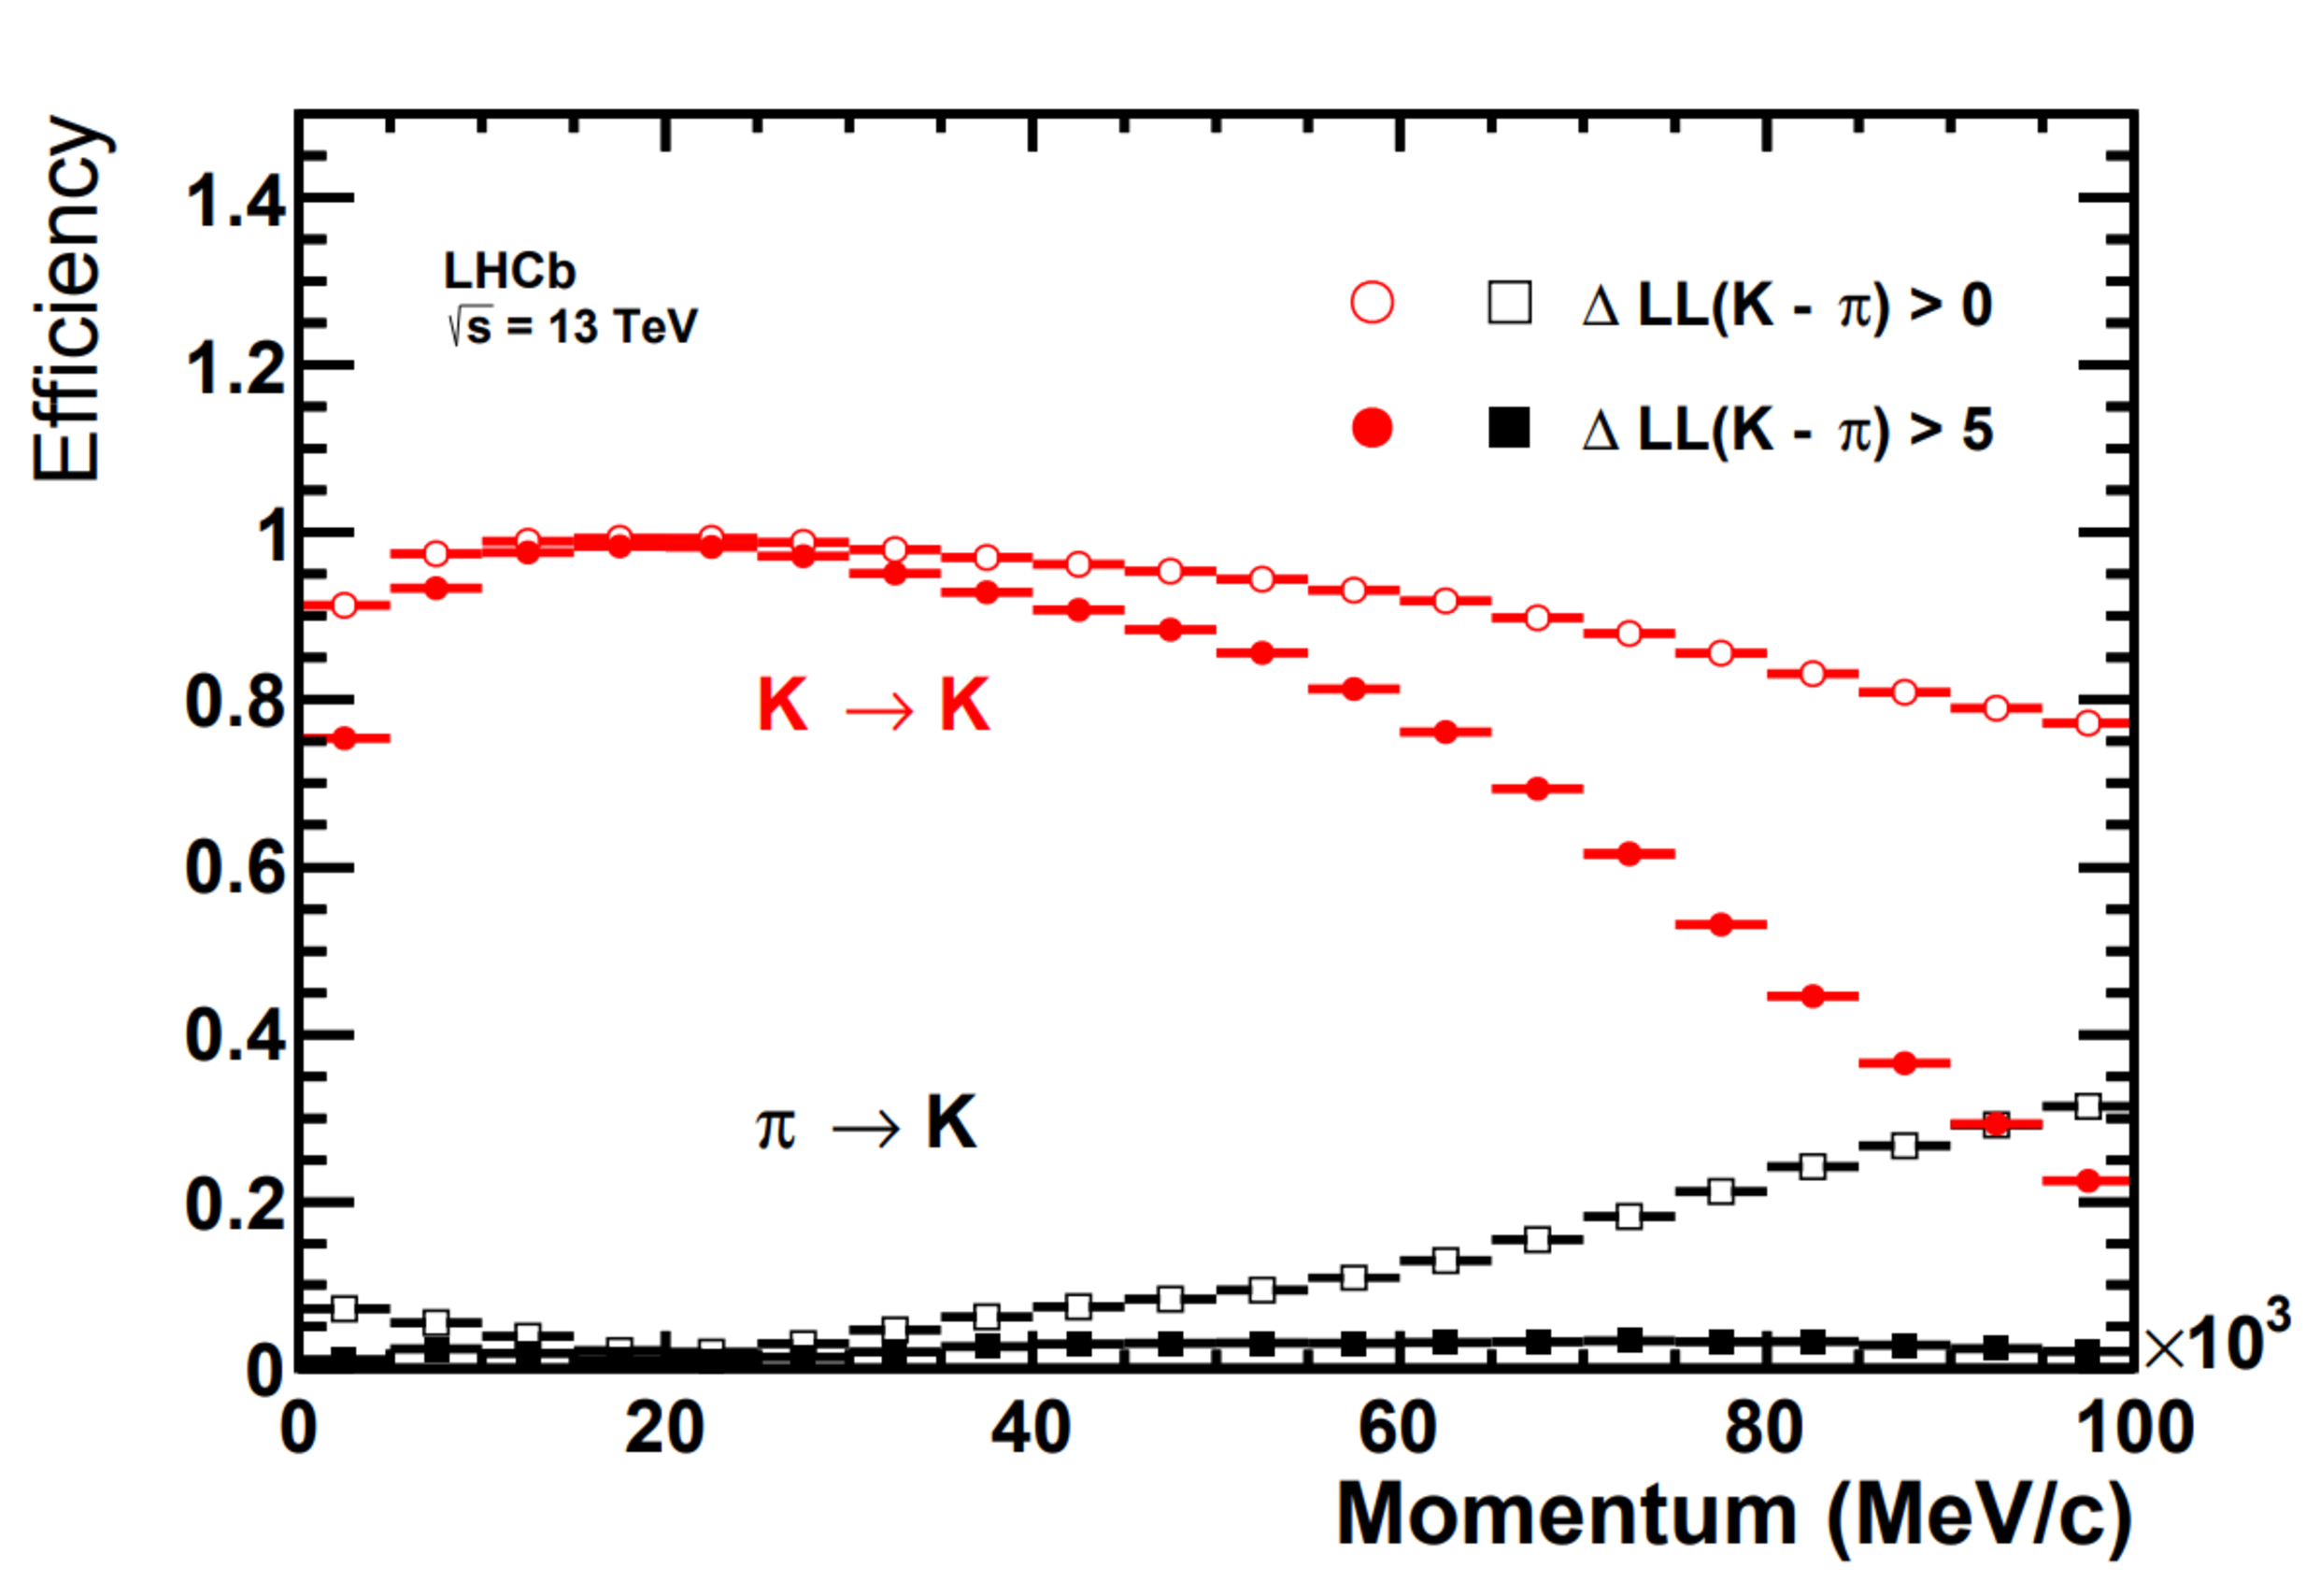
\includegraphics[width=0.5\linewidth]{figures/detector/richperformance_run2.pdf}
\caption{Kaon PID performance of the \rich system as a function of momentum in both \runone (left) and \runtwo (right), showing the efficiency to correctly identify kaons (red points) and the corresponding pion misidentification probability (black points). The expression $\Delta \text{LL}(K - \pi)$ is equivalent to $\log{\mathcal{L}_K} - \log{\mathcal{L}_{\pi}}$, described in the text. Reproduced from Ref \cite{richrun2}.}
\label{richperformance}
\end{figure}

\section{Calorimeters}

The \lhcb calorimeter system provides energy measurements and is essential for the first level of the trigger to select particles with high transverse energy. It consists of four sub-systems: the scintillating-pad (SPD) and pre-shower (PS) detectors, the electromagnetic calorimeter (ECAL) and the hadronic calorimeter (HCAL)~\cite{LHCb-DP-2013-004}. All subsystem components provide energy measurements using the mechanism of detecting scintillation light using photomultiplier tubes (PMTs). The calorimeter system is located downstream of RICH 2, between the first two muon stations, as shown in \fig\ref{lhcbdetector}. The ECAL is required to measure electrons and photons and the HCAL to measure charged and neutral hadrons.  The SPD/PS detectors are nearest the interaction point and designed to help the ECAL with electron identification. Between the SPD and PS is a 15~\mm lead converter, 2.5 radiation lengths thick, to initiate showering before the PS. 

The ECAL is composed of 4~\mm thick alternating lead absorber and polystyrene scintillator layers with an acceptance of 300~mrad horizontally and 250~mrad vertically. The thickness of the ECAL corresponds to 25 radiation lengths, chosen to fully contain high energy photon showers for optimum energy resolution. The energy resolution of the ECAL is parameterised by $\sigma E/E = (8.5-9.5\%)/\sqrt{E} \oplus 0.8\%$, for energy, $E$, in \gev~\cite{calo_latest}.

The HCAL has its scintillating tiles mounted parallel to the beam axis to increase the contact area between the scintillator tiles and optical fibres, maximising the amount of scintillation light collected. The tiles are separated by 100~m thick iron absorber plates. Due to space limitations, the HCAL has a thickness limited to 5.6 nuclear interaction lengths. The measured energy resolution is $\sigma_E/E = (69 \pm 5)\%/\sqrt{E} \oplus (9 \pm 2)\%$ for energy, $E$, in \gev~\cite{calo_latest}.

All four components of the calorimeter system are composed of scintillator pads with a cell granularity that decreases when moving outwards from the beam pipe, as shown in \fig\ref{calorimeter}. The SPD/PS and ECAL have variable segmentation split into three sections, whereas the HCAL is split into two zones with larger cell sizes due to the larger size of hadronic showers.

\begin{figure}
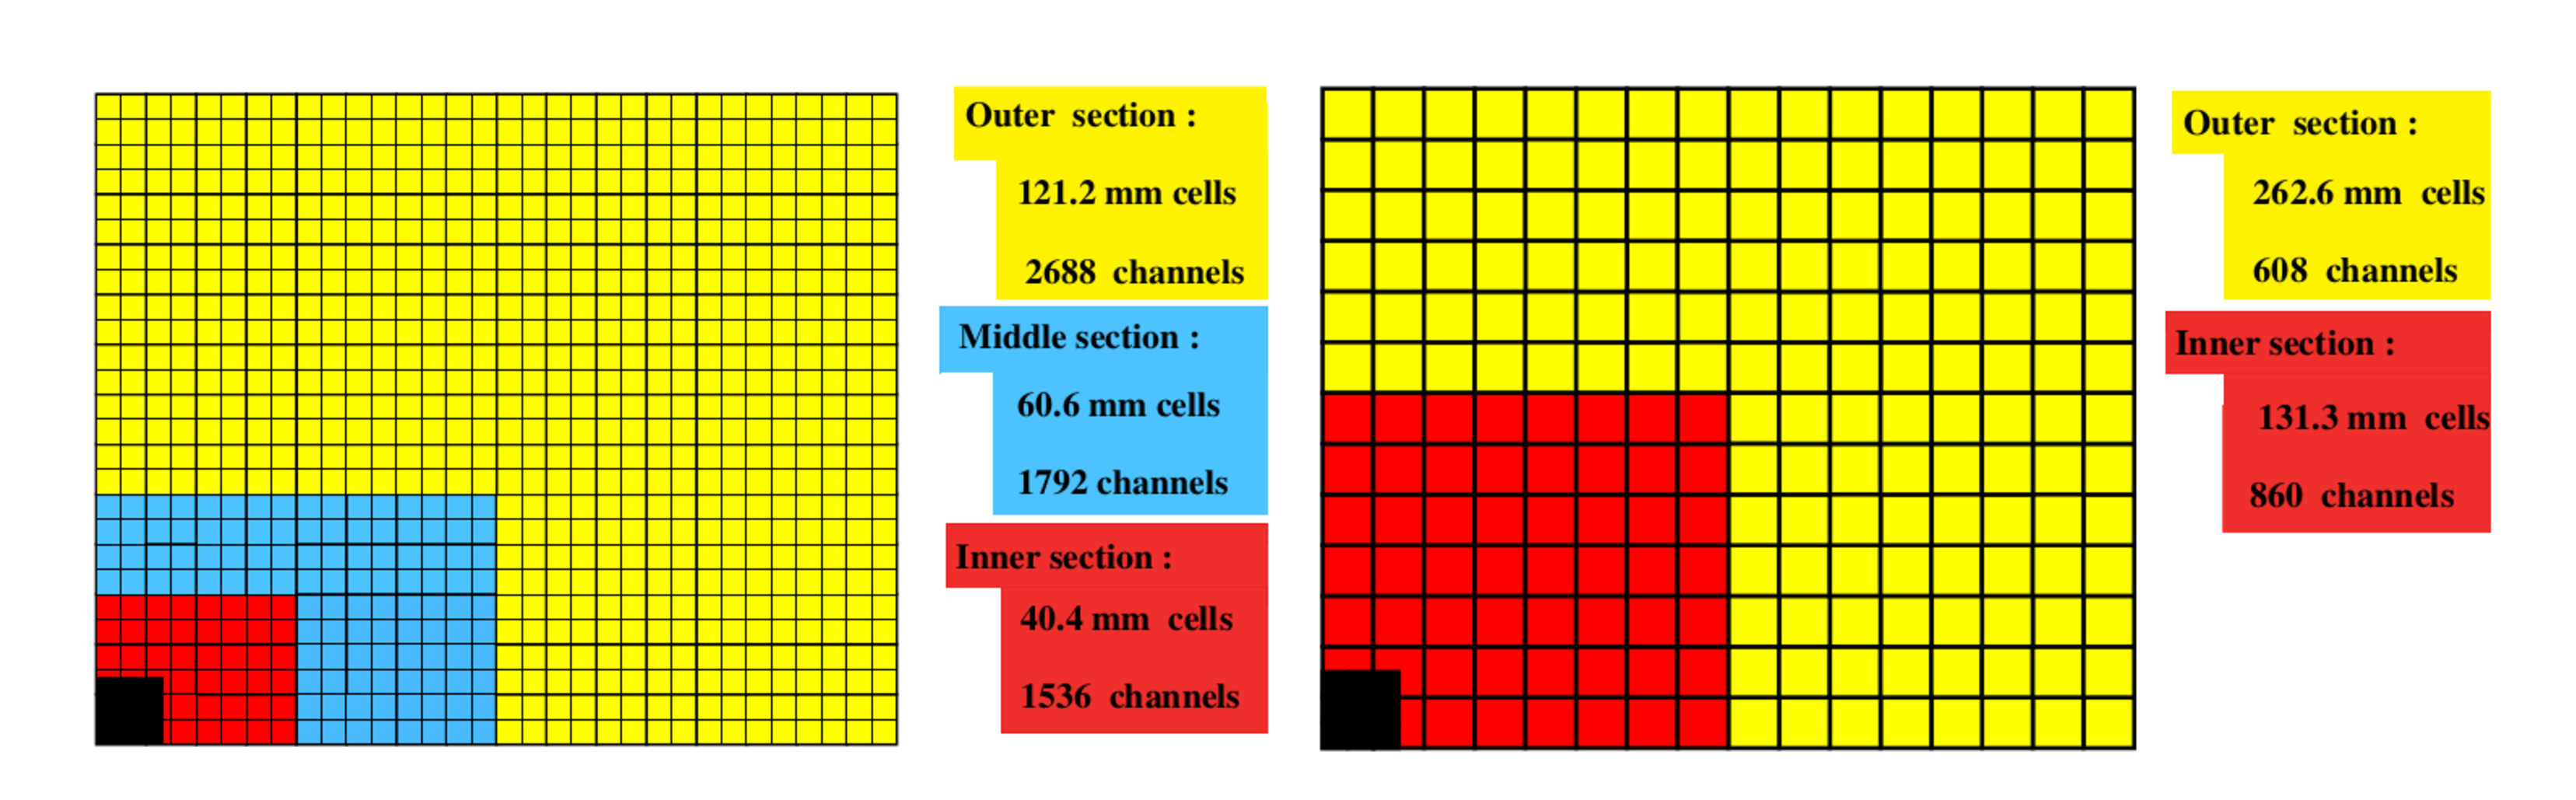
\includegraphics[width=\linewidth]{figures/detector/calorimeters.pdf}
\caption{Segmentation of the SPD/PS and ECAL (left) and the HCAL (right). One quarter of the detector face is shown. Reproduced from Ref.~\cite{lhcbdetector2008}.}
\label{calorimeter}
\end{figure}

\section{Muon system}
\label{sec:detector:muon}

The muon system~\cite{LHCb-DP-2013-001,LHCb-DP-2012-002} is designed, together with the calorimeter system, to provide initial information on whether to accept or reject the event to the first level of hardware trigger, described in \sect\ref{sec:detector:trigger}. The muon system is composed of five stations, labelled M1 through to M5, each containing 276 multi-wire proportional chambers (MWPCs), except the inner-most region of M1, subject to the highest level of radiation, contains 12 gas electron multiplier (GEM) detectors. Station M1 is located upstream from the calorimeters and is only used in the first level of trigger. Stations M2 - M5, located downstream from the calorimeters, are interleaved with 80~\cm thick iron absorbers and are designed to identify and trace penetrating muons. For each muon station the segmentation size increases moving outwards from the beam pipe in four distinct regions, such that each region is subject to the same particle flux. The total active area of the muon system is 435~\ma. Muons with momenta greater than 6~\gevc will typically traverse all five stations. The five stations together have a depth corresponding to 20 interaction lengths. 

Part of the first level of trigger involves performing a stand-alone muon track reconstruction, which requires hits in all 5 muon stations and a calculation of the transverse momentum, \pt, of the tracks. Stations M1 to M3 have the best spatial resolution, which is used to find a rough, fast measurement of the muon \pt for use in the first level of the trigger. Stations M1 to M3 measure muon transverse momentum with a resolution of $\sim$20\%. The muon system provides muon identification for trigger and offline reconstruction with an efficiency larger than 95\%~\cite{LHCb-DP-2014-002}.

\section{Trigger system}
\label{sec:detector:trigger}

The \lhc bunch crossing rate is nominally 40MHz, however there is insufficient processing power to read out the full detector and write every event to storage at this frequency. A dedicated trigger system~\cite{LHCb-DP-2012-004} is therefore implemented to retain interesting events while discarding background events. Triggering occurs in two stages: the low-level hardware trigger using momentum and transverse momentum discrimination, called the Level-0 (L0) trigger, and the high-level software trigger reconstructing the full event, including tracks, called the High Level trigger (HLT). The L0 trigger operates at the bunch crossing rate of 40MHz, reducing the event rate to 1MHz. The HLT only processes events that have passed L0, accepting events at a rate of 5kHz in 2012 (3kHz in 2011). The increase in computing resources in \runtwo meant that events pass HLT and are read out to storage at a rate of 12.5kHz.

A sequence of reconstruction algorithms and thresholds defined in the trigger to select a specific decay is called a trigger line, which returns an accept or reject decision. An event is retained only if it passes at least one trigger line in both L0 and HLT.

\subsection{Level-0 trigger}

The L0 trigger only uses information that can be quickly read out from the calorimeter or muon systems, reducing the event rate from 40MHz to 1MHz, and on an L0 accept the full detector is read out. The L0 trigger relies on the fact that the decay products of \B mesons typically have high transverse momenta due to the large \B mass. The L0 trigger selects high transverse energy clusters in the calorimeters resulting from hadrons, photons and electrons, and high transverse momentum muons in the muon system. The trigger also requires a maximum number of SPD hits to reject high multiplicity events which would use excessive processing time in the HLT. 

The trigger creates {\tt L0Hadron}, {\tt L0Photon} or {\tt L0Electron} candidates depending on which calorimeter subsystem the energy has been deposited in. Events containing at least one candidate above a fixed threshold in transverse energy ({\tt L0Global} candidates) are accepted by the L0 trigger. The hadron trigger selects events with transverse energy, \et $>$ 3.68\gev deposited in the hadronic calorimeter, whereas the electron and photon trigger selects events with \et $>$ 3\gev deposited in the electromagnetic calorimeter. Candidates for {\tt L0Muon} or {\tt L0DiMuon} are created based on the hits in the muon systems and the transverse momentum of the candidate. For a single muon, the muon candidate must have \pt $>$ 1.76\gev, and for a pair of muons, the product of their transverse momentum must be above 1.6$\gev^2$~\cite{trigger_tim}.

\subsection{High Level Trigger}

Events accepted by the L0 trigger are held in a buffer to be processed by the HLT, which has two stages: HLT1, performing partial event reconstruction, and HLT2, performing full event reconstruction. 

For HLT1, the event rate has been reduced by the L0 trigger to 1MHz, allowing latency for the full detector then to be read out. Tracks in the \velo are reconstructed and are then used to form primary vertices using at least five tracks. \velo tracks are identified that either have a large IP, or tracks that match to hits in the muon chamber. Poor quality \velo tracks are rejected. The muon candidates have the additional requirements of high momentum (above 6\gevc) and reasonable track quality (\chisqndf below 25). \velo tracks that are selected by their IP or as a muon candidate are reconstructed using information from the OT and IT-stations in order to determine their momentum. This process is known as forward tracking. Minimum momentum and transverse momentum constraints are applied to reduce processing time when fitting each reconstructed track using a Kalman-filter-based track fit. Successfully extended \velo tracks selected by their large IP are required to have a track \chisq less than three~\cite{trigger_tim}.

In HLT2, the further reduction in event rate by HLT1 allows forward tracking to be performed on all \velo tracks with $p > 5\gevc$ and $\pt > 0.5\gevc$. The HLT2 trigger includes lines for selecting \bquark-hadron decays, prompt charm decays and muonic decays. A large proportion of the HLT2 bandwidth goes to topological trigger lines, which are specifically designed to target partially reconstructed \bquark-hadron decays. Tracks are combined one-by-one requiring the distance of closest approach (DOCA) to be less than 2mm, reaching a total of two, three or four tracks, resulting in the {\tt HLT2Topo(N)BodyBDTDecision} trigger lines, with $N = 2,3,4$ particles forming the vertex. Selection requirements are imposed on these lines based on a multivariate Boosted Decision Tree (BDT) classifier, which uses the sum of transverse momenta, minimum transverse momenta, invariant mass, corrected mass, DOCA, impact parameter significance and flight distance \chisq. Here corrected mass, $m_{corr}$, is defined as

\begin{equation}
m_{corr} \equiv \sqrt{m^2 + {| \pt^{miss} |}^2} + \pt^{miss} \text{ ,}
\end{equation}
where $\pt^{miss}$ represents the missing momentum in the transverse direction. This quantity allows for the case where not all final state particles are reconstructed. This multivariate selection is where most of the rejection power is achieved.

Events that pass HLT2 are written to storage at an event rate of 3kHz (2011), 5kHz (2012) or 12.5kHz (2015 and 2016). These events subsequently undergo the full alignment, calibration and reconstruction processing.

\section{Reconstruction}

\subsection{Track reconstruction}
\label{sec:detector:tracks}

Track reconstruction algorithms combine information from all hits from different sub-detectors, e.g. \velo, TT, IT and OT, to form tracks. There are five categories for track classification, shown in \fig\ref{tracktypes}:

\begin{figure}[h]
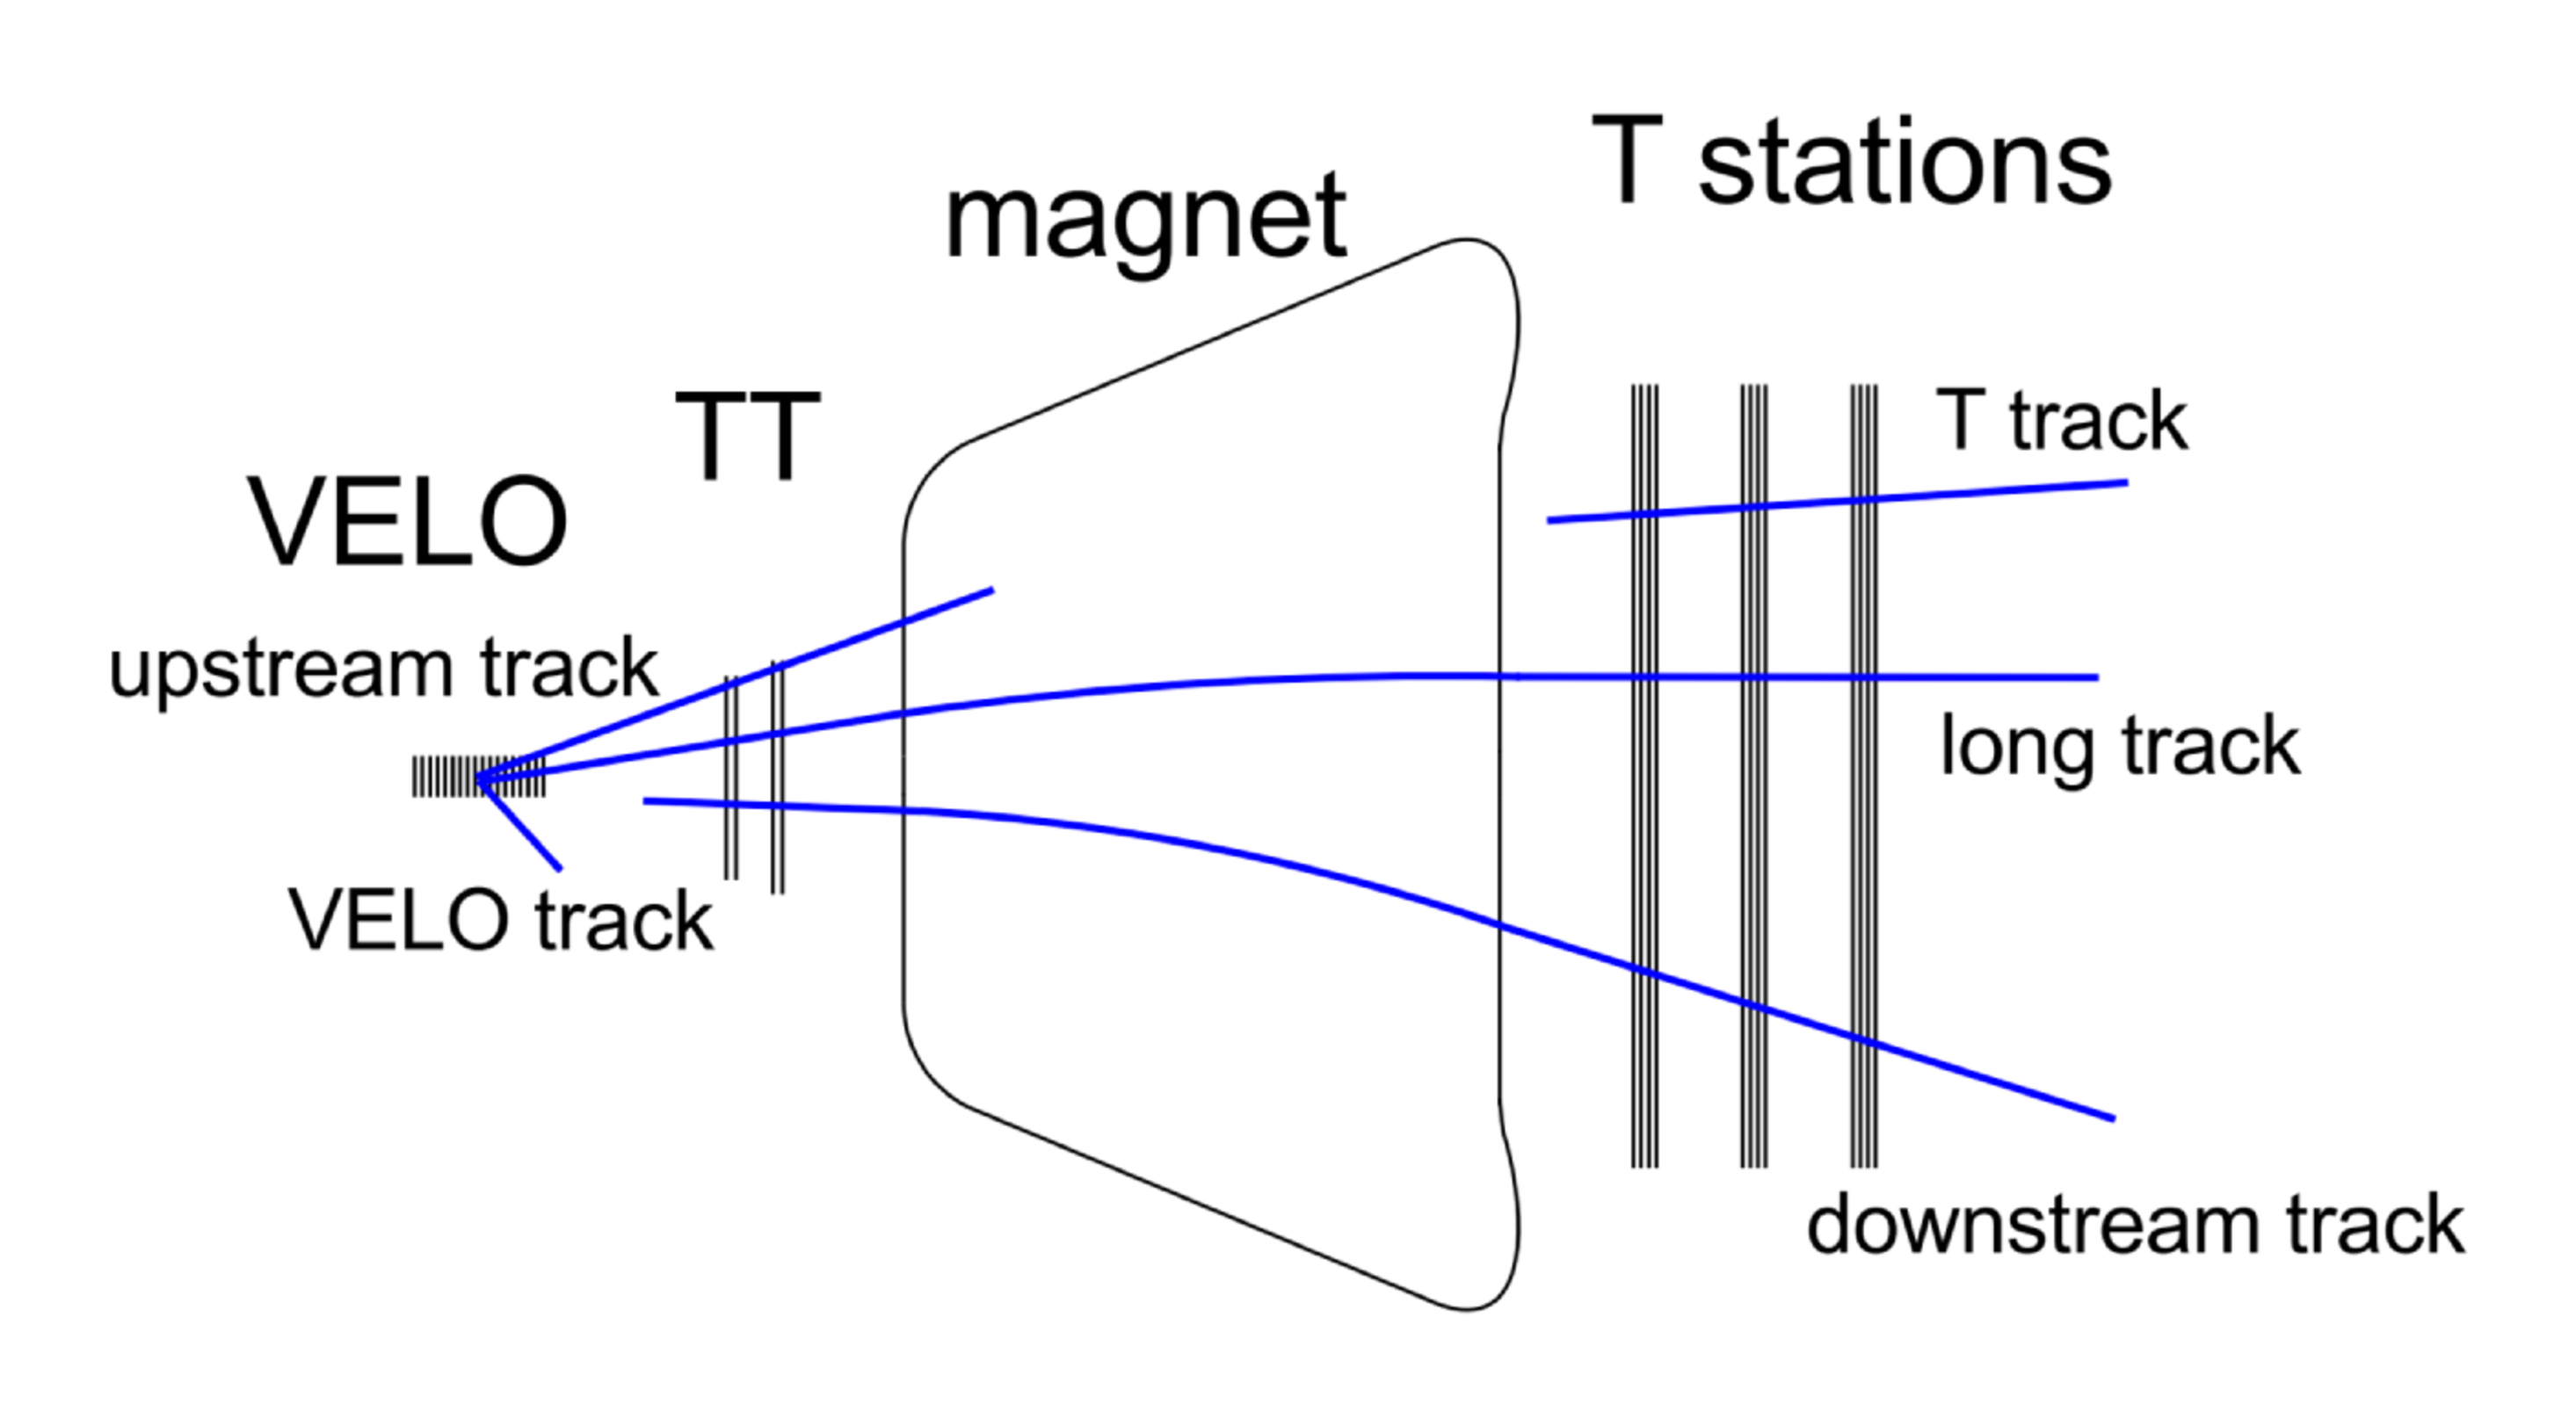
\includegraphics[width=\linewidth]{figures/detector/tracktypes.pdf}
\caption{Schematic diagram of the different tracking sub-detectors (\velo, TT, T-stations) and the different categories of reconstructed tracks (long, downstream, upstream, \velo, T tracks). Reproduced from Ref.~\cite{LHCb-DP-2013-002}.}
\label{tracktypes}
\end{figure}
%1412.6352 figure 14

\begin{itemize}
\item \textbf{Long tracks} traverse the entire tracking system from the \velo to the T-stations. These tracks have the most precise momentum measurement as they have traversed all detector planes and the full magnetic field.
\item \textbf{Downstream tracks} only traverse the TT and T-stations. These tracks are usually a result of long-lived particles, such as \KS mesons, decaying after the \velo.
\item \textbf{Upstream tracks} traverse the \velo and TT stations before being bent out of the detector by the magnetic field due to their lower momentum.
\item \textbf{\velo tracks} leave the \lhcb acceptance after traversing part of the \velo. No momentum information can be obtained from these tracks due to the absence of a magnetic field in this region.
\item \textbf{T tracks} are ones that only have hits in the T-stations. These are typically produced in secondary interactions.
\end{itemize}

Track reconstruction starts with the reconstruction of \velo tracks, which are then propagated through to the TT to determine the particle trajectory. To define a long track, additional hits are searched for in the T-stations that match the particle trajectory. This process finds combinations of clusters in different sub-detectors that are likely to have been formed by a single charged particle travelling though the detector. The sequence of clusters are then fit using a \chisq minimisation procedure with a third order polynomial. Downstream tracks are reconstructed by first searching for T tracks and then finding corresponding hits upstream in the TT by extrapolating the track trajectory back through the magnetic field.

Once the tracks have been identified they are fitted to obtain a best estimate of the track parameters accounting for multiple scattering and energy lost through ionisation. The \chisq of this fit and a neural network classifier are used to reduce the number of fake tracks that are formed by wrongly matching clusters in different sub-detectors, and therefore do not correspond to the passage of a real charged particle.

\subsection{Stripping}
\label{sec:detector:stripping}

The events accepted by the HLT are written to storage. All processing that occurs after this point is known as ``offline'' processing. The events written to storage are processed with more accurate alignment and calibration of the sub-detectors and more sophisticated reconstruction software than HLT. This offline processing stage is referred to in this thesis as ``stripping''. Each family of decays has its own stripping line, which refers to the reconstruction and selection of specified particles in the decay chain of interest. Various loose selection requirements are applied to remove background events to later reduce the processing time and storage requirements. An analysis initially involves taking events returned by the relevant stripping line and developing a more sophisticated selection procedure to further remove background events.

\section{Simulation}

Various simulated samples used in this thesis were generated for signal and background studies. The simulated samples are generated using the \lhcb application \gauss and \boole, which are written using the \gaudi framework~\cite{LHCb-PROC-2011-006,simulation}. \gauss generates particles and their decays as well as simulating the transport of charged and neutral tracks through the detector. \boole is then used to simulate the detector response~\cite{simulation}. 

In the production of simulation samples used for analysis, the first step is the production of \bquark\bquarkbar pairs from $pp$ collisions using \pythia 8~\cite{Sjostrand:2007gs}. One quark in the \bquark\bquarkbar pair is chosen at random to decay via user-specified process and its decay is simulated using \evtgen~\cite{Lange:2001uf}, with \photos~\cite{Golonka:2005pn} modelling any final state radiation. The transport of the decay through the detector is modelled using \geant. \boole then returns the output in the format of real data coming from the front-end electronics. The simulated data are then processed by the trigger, reconstruction and stripping as for real data.

Both magnet polarities, and 2011, 2012, 2015 and 2016 samples are generated with \pythia 8, with all daughter products inside the \lhcb acceptance. Signal samples are simulated \btodkst decays to various \D final states, and with the \Kstarm forced to decay to \KS$\pim$. For the four-body \D final states, the simulated samples are produced assuming the \D decay is uniform over the whole phase space. Various other samples are generated to investigate possible background decays, described in \sect\ref{sec:backgrounds}.
